\documentclass[a4paper,twoside]{article}
\usepackage[T1]{fontenc}
\usepackage[bahasa]{babel}
\usepackage{graphicx,caption}
\usepackage{graphics}
\usepackage{float}
\usepackage[cm]{fullpage}
\pagestyle{myheadings}
\usepackage{etoolbox}
\usepackage{setspace} 
\usepackage{lipsum} 
\setlength{\headsep}{30pt}
\usepackage[inner=2cm,outer=2.5cm,top=2.5cm,bottom=2cm]{geometry} %margin
% \pagestyle{empty}

\makeatletter
\renewcommand{\@maketitle} {\begin{center} {\LARGE \textbf{ \textsc{\@title}} \par} \bigskip {\large \textbf{\textsc{\@author}} }\end{center} }
\renewcommand{\thispagestyle}[1]{}
\markright{\textbf{\textsc{Laporan Perkembangan Pengerjaan Skripsi\textemdash Sem. Ganjil 2018/2019}}}

\onehalfspacing
 
\usepackage[plainpages=false,pdfpagelabels,unicode]{hyperref}
\usepackage{listings}
\usepackage[table]{xcolor}
\hypersetup{unicode=true,colorlinks=true,linkcolor=black,citecolor=black,filecolor=black, urlcolor=black} 

\lstdefinelanguage{JavaScript}{
  keywords={new, true, false, function, return, null, catch, switch, var, if, while, do, else, const, this,Math},
  keywordstyle=\color{blue}\bfseries,
  ndkeywords={moveTo,lineTo,arc,random,floor},
  ndkeywordstyle=\color{purple}\bfseries,
  identifierstyle=\color{black},
  sensitive=false,
  comment=[l]{//},
  morecomment=[s]{/*}{*/},
  commentstyle=\itshape\color{green},
  stringstyle=\color{red},
  morestring=[b]',
  morestring=[b]",
  captionpos=b,
}

\lstset{
   language=JavaScript,
   backgroundcolor=\color{white},
   extendedchars=true,
   basicstyle=\fontfamily{fvm}\selectfont\small, 
   showstringspaces=false,
   showspaces=false,
   numbers=left,
   numberstyle=\footnotesize,
   numbersep=5pt,
   tabsize=4,
   breaklines=true,
   showtabs=false,
   captionpos=b,
   frame=leftline,
   stepnumber=1,
   literate={-}{-}1{-\,-}{--}1
} 

\graphicspath{{../DokumenSkripsi/Gambar/}}% folder tempat gambar 

\begin{document}

\title{\@judultopik}
\author{\nama \textendash \@npm} 

%ISILAH DATA BERIKUT INI:
\newcommand{\nama}{Evelyn Wijaya}
\newcommand{\@npm}{2015730030}
\newcommand{\tanggal}{19/11/2018} %Tanggal pembuatan dokumen
\newcommand{\@judultopik}{Open Source Snake 360} % Judul/topik anda
\newcommand{\kodetopik}{PAN4502}
\newcommand{\jumpemb}{1} % Jumlah pembimbing, 1 atau 2
\newcommand{\pembA}{Pascal Alfadian Nugroho}
\newcommand{\pembB}{-}
\newcommand{\semesterPertama}{45 - Ganjil 18/19} % semester pertama kali topik diambil, angka 1 dimulai dari sem Ganjil 96/97
\newcommand{\lamaSkripsi}{1} % Jumlah semester untuk mengerjakan skripsi s.d. dokumen ini dibuat
\newcommand{\kulPertama}{Skripsi 1} % Kuliah dimana topik ini diambil pertama kali
\newcommand{\tipePR}{B} % tipe progress report :
% A : dokumen pendukung untuk pengambilan ke-2 di Skripsi 1
% B : dokumen untuk reviewer pada presentasi dan review Skripsi 1
% C : dokumen pendukung untuk pengambilan ke-2 di Skripsi 2

% Dokumen hasil template ini harus dicetak bolak-balik !!!!

\maketitle

\pagenumbering{arabic}

\section{Data Skripsi} %TIDAK PERLU MENGUBAH BAGIAN INI !!!
Pembimbing utama/tunggal: {\bf \pembA}\\
Pembimbing pendamping: {\bf \pembB}\\
Kode Topik : {\bf \kodetopik}\\
Topik ini sudah dikerjakan selama : {\bf \lamaSkripsi} semester\\
Pengambilan pertama kali topik ini pada : Semester {\bf \semesterPertama} \\
Pengambilan pertama kali topik ini di kuliah : {\bf \kulPertama} \\
Tipe Laporan : {\bf \tipePR} -
\ifdefstring{\tipePR}{A}{
			Dokumen pendukung untuk {\BF pengambilan ke-2 di Skripsi 1} }
		{
		\ifdefstring{\tipePR}{B} {
				Dokumen untuk reviewer pada presentasi dan {\bf review Skripsi 1}}
			{	Dokumen pendukung untuk {\bf pengambilan ke-2 di Skripsi 2}}
		}
		
\section{Latar Belakang}
\textit{Snake} merupakan sebuah permainan yang pertama kali dibuat oleh Peter Trefonas pada tahun 1978. Konsep \textit{Snake} berasal dari permainan arkade yaitu \textit{Blockade}. Awalnya \textit{Snake} hanya dapat dimainkan pada komputer pribadi. Namun pada tahun 1997, \textit{Snake} dapat dimainkan pada telepon genggam \textit{Nokia}\footnote{https://en.wikipedia.org/wiki/Snake\_(video\_ game\_ genre)}. Cara bermain \textit{Snake} adalah pemain menggerakan ular pada sebuah labirin. Ular tersebut harus mendapatkan makanan sebanyak-banyaknya tanpa menabrak dinding atau ular itu sendiri. Setiap memakan makanan, tubuh ular akan memanjang dan pemain akan semakin sulit untuk menggerakan ular tersebut dengan bebas karena tubuh ular semakin lama akan menutupi labirin tersebut. \\

HTML(\textit{Hyper Text Markup Language}) adalah sebuah bahasa markah yang digunakan untuk membuat halaman web. HTML5 merupakan HTML versi 5 yang terbaru dan penerus dari HTML4, XHTML1, dan DOM level 2 HTML. HTML5 memiliki beberapa elemen baru, salah satunya adalah HTML5 Canvas. HTML5 Canvas adalah tempat untuk menggambar \textit{pixel-pixel} yang dapat ditulis menggunakan bahasa pemrograman \textit{JavaScript}. \textit{Javascript} adalah bahasa pemrograman tingkat tinggi yang digunakan untuk membuat halaman web menjadi lebih interaktif. \textit{GitHub} adalah layanan \textit{web hosting} bersama untuk proyek pengembangan perangkat lunak yang menggunakan sistem \textit{version control} yaitu \textit{Git}. Dengan adanya \textit{Github}, \textit{programmer} dapat mengetahui perubahan yang pada \textit{repository} tersebut. \\

Pada permainan \textit{Snake}, umumnya pergerakan ular hanya atas, bawah, kiri, dan kanan saja. Pada skripsi ini, penulis akan membuat permainan \textit{Snake} yang ularnya dapat bergerak ke segala arah dan orang lain dapat menambahkan labirin menggunakan mekanisme \textit{pull request Github}. Dengan begitu, orang lain dapat menambahkan labirin sesuai dengan keinginanya dan pemain tidak akan cepat bosan karena labirin yang disediakan cukup banyak dan variatif.

\section{Rumusan Masalah}
Rumusan dari masalah yang akan dibahas pada skripsi ini adalah sebagai berikut:
\begin{itemize}
	\item Bagaimana membangun permainan \textit{Snake} menggunakan HTML5?
	\item Bagaimana cara menyimpan labirin pada file eksternal?
	\item Bagaimana cara menggunakan \textit{pull request} pada \textit{Github} agar orang lain dapat menambahkan labirin?
\end{itemize}

\section{Tujuan}
Tujuan-tujuan yang hendak dicapai melalui penulisan skripsi ini adalah sebagai berikut:
\begin{itemize}
	\item Dapat membangun permainan \textit{Snake} menggunakan HTML5.
	\item Dapat menyimpan labirin pada file eksternal.
	\item Dapat menggunakan \textit{pull request} pada \textit{Github} agar orang lain dapat menambahkan labirin.
\end{itemize}

\section{Detail Perkembangan Pengerjaan Skripsi}
Detail bagian pekerjaan skripsi sesuai dengan rencana kerja/laporan perkembangan terakhir :
	\begin{enumerate}
		\item \textbf{Melakukan studi literatur tentang HTML5, \textit{JavaScript}, \textit{jQuery} dan \textit{Git}.}\\
		{\bf Status :} Ada sejak rencana kerja skripsi.\\
		{\bf Hasil :} 

\begin{itemize}
\item \textbf{HTML5 \textit{Canvas}}

HTML5 Canvas adalah sebuah daerah \textit{bitmap} yang dapat dimanipulasi oleh \textit{Javascript}. Pada daerah \textit{bitmap} tersebut, \textit{pixel-pixel} akan di\textit{render} oleh canvas. Setiap \textit{frame}, HTML5 Canvas akan menggambar pada area \textit{bitmap} tersebut menggunakan \textit{Canvas} API(\textit{Application Programming Interface}) yang dipanggil pada \textit{Javascript}. API dari HTML5 Canvas yang umum adalah 2D \textit{Context}. Dengan adanya 2D \textit{Context}, \textit{programmer} dapat membuat bentuk 2D, menampilkan gambar, \textit{render} tulisan, memberi warna, membuat garis dan kurva, dan manipulasi \textit{pixel}. HTML5 Canvas tidak hanya digunakan untuk menggambar dan menampilkan gambar serta tulisan. HTML5 Canvas dapat digunakan untuk membuat animasi, aplikasi pada \textit{web} dan permainan. 

Untuk menambahkan \textit{canvas} pada halaman HTML, diperlukan \textit{tag} <canvas>. Di bawah ini adalah potongan kode untuk menambahkan \textit{canvas} pada halaman HTML. 

\begin{lstlisting}[language=HTML, caption=Menambahkan \textit{canvas}]
	<canvas id='canvas' width='500' height='300'>
		Your browser does not support HTML5 Canvas.
	</canvas>
	
\end{lstlisting}

Diantara tag <canvas> dan </canvas>, dapat dituliskan text yang akan ditampilkan jika browser tidak support HTML5 Canvas.\\
		
\item \textbf{\textit{Javascript}}

\textit{Javascript} adalah bahasa pemrograman yang ringan, \textit{interpreted} dan berorientasi objek yang digunakan pada halaman \textit{web}. \textit{Javascript} dapat membuat objek dengan menambahkan \textit{method} dan atributnya sama seperti bahasa pemrograman C++ dan \textit{Java}. Setelah objek diinisialisasi, maka objek tersebut dapat dijadikan \textit{blueprint} untuk membuat objek lain yang mirip. \textit{Javascript} dapat digunakan untuk mengimplementasi hal yang kompleks pada halaman web. Contohnya adalah menamplikan peta yang interaktif dan membuat animasi 2D/3D. Selain \textit{Javascript}, HTML(\textit{HyperText Markup Language}) dan CSS(\textit{Cascading Style Sheet}) merupakan bagian/komponen penting dalam pembuatan halaman \textit{web}.\\

Untuk menambahkan Javascript pada sebuah halaman web yang dibuat, gunakan tag <script>. Ada 2 cara untuk menambahkan Javascript yaitu menambahkan langsung di halaman web tersebut(Internal Javascript) dan menambahkan file Javascript terpisah(External Javascript).\\

\textbf{Variabel}\\
Variabel adalah sebuah wadah untuk menyimpan nilai/\textit{value}. Untuk mendeklarasi variable pada \textit{Javascript}, digunakan \textit{keyword 'var'}. Variabel pada Javascript tidak perlu menuliskan tipe datanya ketika mendeklarasikan variabel. Hal ini dikarenakan variabel pada Javascript dapat mencakup semua tipe data. Di bawah ini adalah potongan kode untuk mendeklarasikan variabel.

\begin{lstlisting}[language=Javascript, caption=Deklarasi variabel]
	var myVariable = 3;
	
\end{lstlisting}

\textbf{\textit{Constant}}\\
\textit{Constant} adalah sebuah variabel \textit{read-only}, artinya nilai pada \textit{constant} tidak dapat diubah. Untuk mendeklarasikan \textit{constant}, digunakan \textit{keyword 'const'}.\\

\textbf{\textit{Function}}\\
\textit{Function} adalah sekumpulan perintah/\textit{statements} untuk menjalankan suatu tugas atau menghitung nilai. Untuk membuat \textit{function}, digunakan \textit{keyword 'function'}, kemudian diikuti dengan nama \textit{function} tersebut, parameter yang dituliskan di dalam kurung, dan \textit{statement}/perintah \textit{Javascript} yang ditulis di dalam kurung kurawal. Parameter pada \textit{function} bisa lebih dari 1 yang penulisanya dipisahkan oleh tanda koma (,). \textit{Function} bisa memiliki parameter atau tidak. Di bawah ini adalah potongan kode untuk membuat \textit{function} penjumlahan 2 buah bilangan.

\begin{lstlisting}[language=Javascript, caption=\textit{Function} penjumlahan 2 buah bilangan]
	function penjumlahan(angka1,angka2){
		var hasil = angka1+angka2;
		return hasil;
	}
	
\end{lstlisting}

Setelah membuat \textit{function}, \textit{function} tersebut tidak langsung dieksekusi. Membuat \textit{function} hanya memberi nama \textit{function} tersebut dan mendeskripsikan apa yang akan dilakukan oleh \textit{function} tersebut apabila dipanggil. Dengan memanggil \textit{function}, maka \textit{function} akan dieksekusi. Di bawah ini adalah potongan kode untuk memanggil \textit{function} dengan nama penjumlahan.

\begin{lstlisting}[language=Javascript, caption=Memanggil \textit{function} penjumlahan]
	penjumlahan(10,5);
	
\end{lstlisting}

\textbf{Menggambar pada \textit{Canvas}}\\
Sesudah menuliskan \textit{tag} <canvas> pada HTML, canvas tidak bisa langsung digambar. Karena itu perlu ditambahkan \textit{drawing context} pada \textit{Javascript}. Di bawah ini adalah potongan kode untuk menambahkan \textit{drawing context}.

\begin{lstlisting}[language=Javascript, caption=Menambahkan \textit{drawing context canvas}]
	var myCanvas = document.getElementById('canvas');
	var context = myCanvas.getContext('2d');
\end{lstlisting}

Berdasarkan potongan kode di atas, variabel myCanvas menyimpan objek dengan id = 'canvas'. Id ini mengacu ke objek \textit{canvas} pada HTML yang memilki id bernama canvas. Variabel myCanvas sekarang sudah menyimpan objek \textit{canvas}. Kemudian variabel context menyimpan \textit{drawing context} 2D. Sesudah itu, \textit{canvas} tersebut dapat digambar dengan bentuk 2D, garis, kurva, membuat tulisan, dan menambahkan gambar. Selain untuk menggambar, bentuk-bentuk tersebut dapat diberi warna sesuai dengan keinginan.\\

Untuk menggambar bentuk 2D atau garis, diperlukan koordinat x dan y. Koordinat tersebut akan menempatkan gambar tersebut pada \textit{canvas}. Posisi awal/\textit{origin} pada \textit{canvas} adalah (0,0) yang terletak di ujung kiri atas \textit{canvas}. Gambar~\ref{fig:grid} adalah penempatan kotak biru pada \textit{canvas} terhadap \textit{origin}.

\begin{figure}[H]
	\centering  
	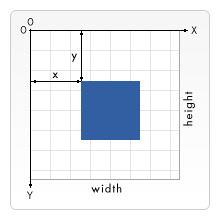
\includegraphics[scale=0.7]{grid}
	\caption[Posisi kotak biru pada \textit{canvas} terhadap \textit{origin}]{Posisi kotak biru pada \textit{canvas} terhadap \textit{origin}}
	\label{fig:grid} 
\end{figure} 

Pada Gambar~\ref{fig:grid}, titik ujung kiri kotak biru tersebut berjarak x \textit{pixel} dari kiri dan berjarak y \textit{pixel} dari atas. \\

\textbf{Menggambar Persegi Panjang}\\
Ada 3 cara untuk menggambar persegi panjang:

\begin{itemize}
	\item \textit{fillRect(x,y,width,height)} : menggambar persegi panjang serta mengisi bagian tengah persegi panjang dengan warna.
	\item \textit{strokeRect(x,y,width,height)} : menggambar \textit{outline} yang berbentuk persegi panjang.
	\item \textit{clearRect(x,y,width,height)} : menghapus daerah yang ditentukan pada \textit{canvas}. Daerah yang dihapus berbentuk persegi panjang.
	\item \textit{rect(x,y,width,height)} : menambah \textit{path} berbentuk persegi panjang.
\end{itemize}

Fungsi tersebut memiliki parameter yang sama. Parameter x dan y untuk menentukan posisi pada canvas dari titik ujung kiri atas persegi panjang. \textit{Width} adalah lebar dari persegi panjang dan \textit{height} adalah tinggi dari persegi panjang.\\

\textbf{Menggambar \textit{Path}}\\
\textit{Path} adalah sekumpulan titik yang dihubungkan oleh segmen garis. \textit{Path} dapat membentuk kurva dan membuat bentuk 2D lainnya seperti segitiga, trapesium, belah ketupat dan lain-lain. Langkah-langkah untuk membuat bentuk menggunakan path adalah sebagai berikut : 
\begin{enumerate}
	\item Buat \textit{path}.
	\item Tuliskan perintah untuk menggambar pada \textit{path} tersebut.
	\item Sesudah \textit{path} tersebut sudah dibuat, \textit{path} tersebut dapat di\textit{render} menggunakan \textit{stroke} atau \textit{fill}.
\end{enumerate}

Langkah pertama untuk membuat \textit{path} baru adalah dengan menggunakan fungsi \textit{beginPath()}. Setelah itu, perintah-perintah untuk menggambar dapat digunakan untuk membuat bentuk-bentuk yang diinginkan. Apabila sudah selesai menggambar, gunakan fungsi \textit{stroke()} untuk menggambar outline dari \textit{path} tersebut atau \textit{fill()} untuk mengisi \textit{area path} tersebut. Setelah itu, gunakan fungsi \textit{closePath()} untuk menutup bentuk tersebut dengan cara menggambar garis lurus dari posisi titik terakhir ke titik awal.\\

Fungsi lainnya yang menjadi bagian dari membuat \textit{path} adalah fungsi \textit{moveTo()}. Fungsi ini diibaratkan seperti mengangkat sebuah pensil dari sebuah titik pada kertas kemudian menempatkanya pada titik yang diinginkan. Fungsi \textit{moveTo()} memiliki 2 parameter yaitu x dan y yang merupakan posisi titik pada \textit{canvas}. Ketika \textit{canvas} sudah diinisialsasi dan fungsi \textit{beginPath()} sudah dipanggil, fungsi \textit{moveTo()} berguna sebagai penempatan titik awal untuk menggambar. Fungsi \textit{lineTo()} memiliki 2 parameter yaitu x dan y yang merupakan titik akhir dari garis. Garis akan digambar mulai dari posisi titik awal sampai ke posisi titik akhir garis. Titik awal ini bergantung pada titik akhir dari \textit{path} sebelumya. Titik awal dapat diubah dengan menggunakan fungsi \textit{moveTo()}.\\

Fungsi \textit{arc()} digunakan untuk menggambar lingkaran atau busur. Fungsi ini memiliki 6 parameter yaitu x, y, radius, \textit{startAngle}, \textit{endAngle} dan \textit{anticlockwise}. Parameter x dan y adalah posisi titik tengah busur pada \textit{canvas}. Radius adalah besar jari-jari busur. \textit{StartAngle} dan \textit{endAngle} adalah titik awal dan titik akhir busur dalam satuan radian yang diukur dari sumbu x. \textit{Anticlockwise} adalah parameter yang bernilai \textit{boolean}, apabila bernilai \textit{true}, maka busur akan digambar berlawanan arah jarum jam dan jika bernilai \textit{false}, busur akan digambar searah jarum jam. Karena fungsi \textit{arc()} menerima input sudut dalam radian, maka perlu dilakukan konversi dari satuan derajat menjadi radian terlebih dahulu. Rumusnya adalah sebagai berikut : \textbf{radian = (Math.PI / 180) * besar sudut}\\

\textit{B\'ezier curve} merupakan tipe \textit{path} yang digunakan untuk membuat kurva. \textit{B\'ezier curve} ada 2 jenis yaitu \textit{cubic} dan \textit{quadratic}. Perbedaanya adalah \textit{quadratic B\'ezier curve} memiliki sebuah \textit{control point}, sedangkan \textit{cubic B\'ezier curve} memiliki 2 buah \textit{control point}. Pada Gambar~\ref{fig:bezier} menunjukkan perbedaan antara \textit{quadratic B\'ezier curve} dan \textit{cubic B\'ezier curve}. Titik merah pada gambar merupakan \textit{control point} dari \textit{B\'ezier curve}.

\begin{figure}[H]
	\centering  
	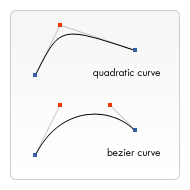
\includegraphics[scale=0.8]{bezier}
	\caption[Perbedaan \textit{quadratic B\'ezier curve} dan \textit{cubic B\'ezier curve}]{Perbedaan \textit{quadratic B\'ezier curve} dan \textit{cubic B\'ezier curve}}
	\label{fig:bezier} 
\end{figure} 

Berikut adalah fungsi \textit{quadratic} dan \textit{cubic B\'ezier curve} :
\begin{itemize}
	\item \textit{quadraticCurveTo(cp1,cp2,x,y)} : menggambar \textit{quadratic B\'ezier curve} dari posisi pensil sekarang ke titik akhir yaitu x dan y, dengan titik control point yaitu cp1 dan cp2.
	\item bezierCurveTo(cp1x,cp1y,cp2x,cp2y,x,y) : menggambar \textit{cubic B\'ezier curve} dari posisi pensil sekarang ke titik akhir yaitu x dan y, dengan 2 titik control point yaitu (cp1x,cp1y) dan (cp2x,cp2y).
\end{itemize}

\textbf{\textit{Object Oriented Programming Javascript}}\\
OOP (\textit{Object Oriented Programming}) adalah sebuah paradigma \textit{programming} yang menggunakan abstraksi untuk membuat objek-objek yang ada pada dunia nyata. Bahasa pemrograman seperti \textit{Java}, C++, \textit{Ruby, Phyton}, PHP, dan \textit{Objective-C} sudah mendukung OOP. Dalam OOP, setiap objek dapat menerima pesan, memproses data dan mengirim pesan ke objek lain. Program yang menggunakan konsep OOP ini mudah untuk dimengerti dan lebih mudah untuk dikembangkan oleh \textit{programmer}. \\

Ide umum pada OOP adalah menggunakan objek untuk memodelkan benda-benda yang ada pada dunia nyata. Objek tersebut kemudian direpresentasi pada program yang dibuat. Objek-objek dapat berisi data, fungsionalitas dan \textit{behaviour} yang merepresentasikan informasi tentang objek tersebut dan tugas objek. Contohnya, membuat objek sebuah mobil. Mobil memiliki beberapa informasi diantaranya adalah merk mobil, berat mobil, warna mobil dan tahun produksi. Informasi tersebut dapat disebut sebagai properti dari objek. Mobil dapat bergerak maju, berbelok ke kanan, berbelok ke kiri, bergerak mundur dan berhenti. Hal-hal yang dapat dilakukan oleh objek disebut sebagai method dari objek. \\

\textbf{Kelas}\\
\textit{Javascript} tidak memiliki \textit{statement 'class'} yang dapat digunakan pada bahasa pemrograman C++ atau \textit{Java}. Untuk membuat kelas, \textit{Javascript} menggunakan \textit{function} sebagai konstruktor untuk kelas. Karena itu, membuat kelas sama dengan membuat \textit{function} pada \textit{Javascript}. Di bawah ini adalah potongan kode untuk membuat kelas bernama Mobil.

\begin{lstlisting}[language=Javascript, caption=Membuat kelas Mobil]
	function Mobil(){}
	
\end{lstlisting}

\textbf{Objek}\\
Untuk membuat instansi baru dari objek, gunakan \textit{statement 'new'} yang nantinya akan disimpan pada variabel. Di bawah ini adalah potongan kode untuk membuat instansi.

\begin{lstlisting}[language=Javascript, caption=Membuat \textit{instance} mobil]
	var mobil1 = new Mobil();
\end{lstlisting}

\textbf{Konstruktor}\\
Konstruktor adalah \textit{method} yang ada pada kelas. Konstruktor akan dipanggil ketika pertama kali inisialisasi atau saat instansi dari objek baru dibuat. \textit{Function} pada \textit{Javascript} berfungsi sebagai konstruktor sehingga tidak perlu membuat method konstruktor lagi. Semua aksi yang terdapat pada kelas akan dieksekusi pada saat instansiasi.\\

\textbf{Properti/Atribut}\\
Properti adalah variabel yang terdapat pada kelas. Properti ditulis pada konstruktor kelas sehingga setiap properti pada kelas akan dibuat ketika membuat instansi baru. Untuk membuat properti, gunakan \textit{statement 'this'}. \textit{Statement 'this'} juga dapat diartikan bahwa atribut-atribut yang dibuat merupakan atribut milik objek. Cara ini mirip dengan bahasa pemrograman \textit{Java} ketika membuat sebuah properti pada objek. Sintaks untuk mengakses properti di luar kelas adalah : namaInstansi.properti. Di bawah ini adalah potongan kode untuk mendefinisikan properti pada kelas Mobil pada saat instansiasi.

\begin{lstlisting}[language=Javascript, caption=Mendefinisikan properti pada kelas Mobil]
	function Mobil(merkMobil,beratMobil,warnaMobil,tahunProduksi){
		this.merkMobil = merkMobil;
		this.beratMobil = beratMobil; //satuan dalam kg
		this.warnaMobil = warnaMobil;
		this.tahunProduksi = tahunProduksi;
	}
	
	var mobil1 = new Mobil('Toyota',1000,'Hitam',2010);
	
\end{lstlisting}

\textbf{\textit{Method}}\\
\textit{Method} adalah hal yang dapat dilakukan oleh sebuah objek. Untuk membuat \textit{method}, tuliskan nama \textit{method} terlebih dahulu kemudian \textit{assign} fungsi pada nama method tersebut. Untuk memanggil \textit{method} sebuah objek, tuliskan nama objek/kelas terlebih dahulu, kemudian tuliskan nama \textit{method} sesuai dengan yang sudah dibuat beserta tanda kurung. Tanda kurung berisi parameter. Di bawah ini adalah potongan kode untuk membuat dan memanggil method bergerakMaju() pada kelas Mobil.

\begin{lstlisting}[language=Javascript, caption=Membuat dan memanggil method bergerakMaju()]
	function Mobil(merkMobil,beratMobil,warnaMobil,tahunProduksi){
		this.merkMobil = merkMobil;
		this.beratMobil = beratMobil; //satuan dalam kg
		this.warnaMobil = warnaMobil;
		this.tahunProduksi = tahunProduksi;
		
		this.bergerakMaju = function(){
			//kode agar mobil bergerak maju
		}
	}
	
	var mobil1 = new Mobil('Toyota',1000,'Hitam',2010);
	mobil1.bergerakMaju(); //memanggil fungsi untuk bergerak maju
	
\end{lstlisting}

\textbf{\textit{Event}}\\
\textit{Event} adalah kejadian/peristiwa yang terjadi pada sistem yang diprogram. Sistem akan memberitahu apabila kejadian tersebut sudah terjadi dan akan melakukan suatu aksi ketika kejadian sudah terjadi. Misalnya, di bandara ketika landasan pacu sudah bersih untuk pesawat lepas landas, sinyal akan dikomunikasikan kepada pilot bahwa pesawat sudah boleh untuk lepas landas. Dalam \textit{web}, \textit{event} ditembakan di dalam \textit{browser window} dan dikaitkan pada objek yang spesifik seperti sekumpulan elemen, dokumen HTML yang dimuat atau keseluruhan \textit{browser window}. Ada beberapa \textit{event} yang dapat terjadi diantaranya adalah : 

\begin{itemize}
	\item Pengguna mengklik sebuah element atau mengarahkan kursor ke sebuah elemen.
	\item Pengguna menekan sebuah tombol pada \textit{keyboard}.
	\item Pengguna mengatur besar dan menutup \textit{browser window}.
	\item Halaman \textit{web} selesai dimuat.
	\item \textit{Form} sedang di\textit{submit}.
	\item Video sedang dimainkan, dijeda, atau selesai.
	\item Ketika \textit{error} terjadi.
\end{itemize}

Setiap \textit{event} memiliki \textit{event handler}, yang berisikan sekumpulan kode yang akan dijalankan ketika \textit{event} sudah terjadi. \textit{Event handler} juga sering disebut sebagai \textit{event listener}. \textit{Listener} menunggu \textit{event} yang terjadi dan \textit{handler} adalah kode yang dijalankan ketika \textit{listener} mendapatkan \textit{event}/ketika \textit{event} terjadi. Untuk memperjelas bagaimana cara menggunakan \textit{event}, di bawah ini terdapat contoh kode untuk menambahkan event pada button/tombol.

\begin{lstlisting}[language=Javascript,{alsolanguage=HTML}, caption=Menambahkan event pada button]
	<html>
		<title>Event pada tombol</title>
		<body>
			<button id='tombol'>Change color</button>
		</body>
	</html>
	
	<script>
		var btn = document.getElementById('tombol');

		function random(number) {
  			return Math.floor(Math.random()*(number+1));
		}

		btn.onclick = function() {
  			var rndCol = 'rgb(' + random(255) + ',' + random(255) + ',' + random(255) + ')';
  			document.body.style.backgroundColor = rndCol;
		}
	</script>
	
\end{lstlisting}

Berdasarkan kode di atas, objek \textit{button} dengan id='tombol' disimpan di dalam variabel bernama 'btn'. Ada fungsi bernama \textit{'random'} untuk mengembalikan sebuah nilai acak. Setelah itu ada \textit{event handler}. \textit{Event handler property} yang digunakan adalah \textit{onclick}. \textit{Event handler property onclick} mengecek apakah objek(dalam kasus ini objeknya adalah button) sudah ditekan/diklik. Bila tombol sudsh diklik, maka akan mengeksekusi fungsi untuk mengubah warna \textit{background}. Warna RGB tersebut di\textit{generate} secara acak menggunakan fungsi \textit{random} yang sudah dibuat sebelumnya. Tidak hanya \textit{event handler property onclick} saja yang dapat digunakan pada halaman web. Berikut ini adalah beberapa \textit{event handler property} lainnya:

\begin{itemize}
	\item \textit{onfocus} dan \textit{onblur} : event akan terjadi apabila sebuah objek difokuskan/tidak. Biasanya digunakan untuk menampilkan informasi tentang bagaimana cara mengisi \textit{form} ketika difokuskan atau menampilkan pesan \textit{error} ketika \textit{form} tersebut diisi dengan nilai yang salah/tidak valid.
	\item \textit{ondblclick} : \textit{event} akan terjadi ketika objek diklik 2 kali/\textit{double click}.
	\item \textit{window.keypress, window.onkeydown, window.onkeyup} : \textit{event} akan terjadi apabila sebuah tombol pada \textit{keyboard} ditekan. \textit{Keypress} adalah \textit{event} ketika tombol ditekan kemudian dilepas. \textit{Keydown} adalah \textit{event} ketika tombol ditekan dan \textit{keyup} adalah \textit{event} ketika tombol dalam keadaan tidak ditekan. Untuk ketiga \textit{event} ini, event tersebut harus di\textit{register} pada objek \textit{window} yang merepresentasikan \textit{browser window}.
	\item \textit{onmouseover} dan \textit{onmouseout} : event akan terjadi ketika posisi kursor \textit{mouse} berada luar objek lalu ditempatkan di atas objek dan ketika posisi kursor \textit{mouse} berada di atas objek lalu keluar dari objek. 
\end{itemize}

Beberapa \textit{event handler property} tersebut sangat umum dan tersedia di manapun, sedangkan beberapa \textit{event handler property} lainnya sangat spesifik dan hanya digunakan untuk elemen tertentu, contohnya adalah menggunakan \textit{onplay} untuk elemen tertentu yaitu <video>.\\

Mekanisme event terbaru dalam spesifikasi DOM(\textit{Document Object Model}) \textit{level} 2 \textit{Events} yang memberikan \textit{browser} sebuah fungsi baru yaitu \textit{addEventListener()}. Fungsi ini mirip seperti \textit{event handler property} namun memiliki sintaks yang berbeda. Di bawah ini adalah potongan kode untuk menggunakan fungsi \textit{addEventListener()}.

\begin{lstlisting}[language=Javascript, caption=Menggunakan fungsi addEventListener()]
	var btn = document.getElementById('tombol');

	function bgChange() {
  		var rndCol = 'rgb(' + random(255) + ',' + random(255) + ',' + random(255) + ')';
  		document.body.style.backgroundColor = rndCol;
	}   

	btn.addEventListener('click', bgChange);
	
\end{lstlisting}

Pada fungsi \textit{addEventListener()}, ada 2 buah parameter yaitu \textit{event} yang ingin digunakan(dalam potongan kode di atas menggunakan \textit{event click}) dan kode sebagai \textit{handler} yang ingin dijalankan ketika \textit{event} tersebut terjadi. Selain cara di atas, dapat juga menuliskan semua kode di dalam fungsi \textit{addEventListener()} seperti potongan kode di bawah ini.

\begin{lstlisting}[language=Javascript, caption=Menuliskan kode di dalam fungsi addEventListener()]
	btn.addEventListener('click', function() {
  		var rndCol = 'rgb(' + random(255) + ',' + random(255) + ',' + random(255) + ')';
  		document.body.style.backgroundColor = rndCol;
	});
	
\end{lstlisting}


\textbf{Membuat Animasi}\\
Langkah-langkah untuk membuat animasi adalah sebagai berikut :

\begin{enumerate}
	\item Membersihkan \textit{canvas} : hilangkan semua bentuk-bentuk yang sudah tergambar di canvas. Untuk menghapus keseluruhan \textit{canvas}, gunakan fungsi \textit{clearRect()}.
	\item Menyimpan \textit{state canvas} : ketika mengubah atribut(seperti \textit{style}) yang mempengaruhi \textit{state canvas} dan ingin \textit{original state} tersebut digunakan kembali, \textit{state} tersebut harus disimpan. 
	\item Gambar bentuk : gambar bentuk yang ingin dianimasikan.
	\item Mengembalikan \textit{state canvas} : jika state sudah disimpan, kembalikan \textit{state} tersebut sebelum menggambar di \textit{frame} yang baru.
\end{enumerate}

Bentuk yang digambar pada \textit{canvas} dapat menggunakan fungsi yang dimiliki oleh \textit{canvas} atau dengan membuat fungsi sendiri. Hasil yang ada pada \textit{canvas} akan muncul setelah \textit{script} selesai dieksekusi. Jadi dibutuhkan cara mengeksekusi fungsi secara terus menerus untuk menggambar dalam waktu tertentu. Ada 3 fungsi yang dapat digunakan untuk memanggil fungsi dalam kurun waktu tertentu diantaranya adalah :

\begin{itemize}
	\item \textit{setInterval(function,delay)}: mengeksekusi fungsi \textit{function} berulang kali setiap \textit{delay} milidetik.
	\item \textit{setTimeout(function,delay)}: mengeksekusi fungsi \textit{function} setiap \textit{delay} milidetik.
	\item \textit{requestAnimationFrame(callback)}: memberitahu \textit{browser} untuk menjalankan animasi dan meminta \textit{browser} memanggil fungsi yang spesifik untuk memperbarui animasi.
\end{itemize}

Jika tidak ingin ada iteraksi user, gunakan fungsi \textit{setInterval()} untuk mengeksekusi fungsi berulang kali. Bila ingin ada interaksi user, terutama dalam pembuatan game yang membutuhkan input \textit{keyboard} atau \textit{mouse} untuk mengontrol animasi, gunakan fungsi setTimeout().\\

\item \textbf{\textit{jQuery}}\\
\textit{jQuery} merupakan \textit{library Javascript}. Semua yang ada pada \textit{jQuery} dapat diakses melalui \textit{Javascript}. Untuk dapat menggunakan \textit{jQuery}, perlu menambahkan \textit{script jQuery} pada tag <script> di bagian \textit{src}. Untuk memanggil objek menggunakan \textit{jQuery} harus diawali simbol \$, kemudian diikuti dengan objek dan \textit{method}nya. Contoh penulisan pada \textit{jQuery} adalah sebagai berikut : \textit{\$("h1").remove().}\\

Sebuah halaman \textit{web} tidak dapat dimanipulasi dengan aman apabila halaman tersebut belum siap. \textit{jQuery} menyediakan \textit{\$(document).ready()} untuk mengecek apakah halaman sudah siap. Kode yang berada di dalam \textit{\$(document).ready()} akan dijalankan oleh \textit{Javascript} setelah halaman DOM(\textit{Document Object Model}) sudah siap dimuat. Berikut adalah potongan kode untuk menuliskan \textit{\$(document).ready()}: 

\begin{lstlisting}[language=Javascript, caption=Menuliskan method \textit{\$(document).ready()}]
	$( document ).ready(function() {
    	//tuliskan kode di bagian ini
	});
\end{lstlisting}

\textit{Method .attr()} berfungsi sebagai \textit{setter} dan \textit{getter}. Sebagai \textit{setter}, \textit{method .attr()} dapat menerima sebuah \textit{key} dan \textit{value} atau sebuah objek yang memiliki satu atau lebih \textit{key/value pair}. Di bawah ini adalah contoh \textit{method} \textit{.attr()} sebagai \textit{setter} dan \textit{getter}.

\begin{lstlisting}[language=Javascript, caption=Method .attr() sebagai setter]
	$( "a" ).attr( "href", "allMyHrefsAreTheSameNow.html" );
 
	$( "a" ).attr({
    title: "all titles are the same too!",
    href: "somethingNew.html"
});
\end{lstlisting}

\begin{lstlisting}[language=Javascript, caption=Method .attr() sebagai getter]
	$( "a" ).attr( "href" ); //mengembalikan href yang memiliki elemen a pertama pada dokumen
});
\end{lstlisting}

Konsep yang paling umum pada \textit{jQuery} adalah menyeleksi beberapa elemen dan melakukan sesuatu terhadap elemen tersebut. Ada beberapa cara untuk menyeleksi beberapa elemen diantaranya adalah sebagai berikut:

\begin{itemize}
	\item \textit{\$( "\#myId" )} : mendapatkan elemen berdasarkan id. Id harus unik per halaman.
	\item \textit{\$( ".myClass" )} : mendapatkan elemen berdasarkan nama kelas.
	\item \textit{\$( "input[name='first\_name']" )} : mendapatkan elemen berdasarkan atributnya.
	\item \textit{\$( "\#contents ul.people li" )} : mendapatkan elemen berdasarkan \textit{Compound CSS Selector}.
	\item \textit{\$( "div.myClass, ul.people" )} : mendapatkan elemen berdasarkan sekumpulan \textit{selector}.
\end{itemize} 

Untuk mengecek apakah elemen tidak kosong, maka cek elemen tesebut dengan menggunakan \textit{method .length()}. Apabila nilai tersebut 0, maka elemenya kosong. \textit{jQuery} tidak menyimpan elemen. Untuk itu dibutuhkan variabel untuk menyimpan elemen tersebut jika ingin mendapatkan elemen lain. Di bawah ini adalah potongan kode untuk menyimpan elemen pada variabel.

\begin{lstlisting}[language=Javascript, caption=Menyimpan elemen pada variabel]
	var divs = $( "div" );
});
\end{lstlisting}

Beberapa \textit{method} pada \textit{jQuery} dapat digunakan untuk mendapatkan atau me-\textit{assign} nilai pada saat seleksi. Ketika \textit{method} dipanggil dengan sebuah nilai sebagai argumen, \textit{method} tersebut dapat disebut sebagai \textit{setter}. Ketika method dipanggil tanpa argumen, method tersebut mendapatkan nilai dari elemen/sebagai \textit{getter}.

\begin{lstlisting}[language=Javascript, caption=Setter dan getter]
	$( "h1" ).html( "hello world" ); //assign elemen h1 dengan 'hello world'
	$( "h1" ).html(); // mendapatkan nilai elemen h1 pertama
});
\end{lstlisting}

Ada beberapa cara untuk mengubah elemen yang ada. Cara yang paling umum adalah mengubah \textit{inner HTML} atau atribut dari sebuah elemen. \textit{jQuery} menyediakan \textit{method-method} untuk menngubah/memanipulasinya. Cara ini juga dapat digunakan untuk mendapatkan informasi tentang elemen tersebut. Di bawah ini adalah beberapa method yang digunakan untuk mendapatkan dan mengubah informasi dari elemen :

\begin{itemize}
	\item \textit{.html()} : mendapatkan atau mengubah konten HTML.
	\item \textit{.text()} : mendapatkan atau mengubah konten tulisan.
	\item \textit{.attr()} : mendaptakan atau mengubah nilai atribut yang diinginkan
	\item \textit{.width()} : mendapatkan atau mengubah lebar sebuah elemen.
	\item \textit{.height()} : mendapatkan atau mengubah tinggi sebuah elemen.
	\item \textit{.position()} : mendapatkan posisi sebuah objek. Method ini tidak dapat digunakan untuk mengubah nilai.
	\item \textit{.val()} : mendapatkan atau mengubah nilai dari elemen pada \textit{form}. 
\end{itemize} 

\textbf{\textit{Events}}\\
\textit{jQuery} dapat mengatur \textit{event} pada halaman \textit{web}. \textit{Event} ini biasanya akan terjadi apabila ada interaksi pengguna dengan halaman \textit{web}, misalnya ketika mengisi teks pada \textit{form} atau kursor pada mouse dipindahkan. \textit{jQuery} menyediakan \textit{method event} untuk \textit{native browser}, diantaranya adalah \textit{.click(), .focus(), .blur(), .change()} dan masih banyak lagi. Selain itu method \textit{.on()} berguna untuk \textit{binding} fungsi \textit{handler} yang sama untuk banyak \textit{event}. Di bawah ini adalah contoh potongan kode \textit{event jQuery}.

\begin{lstlisting}[language=Javascript, caption=Event click ]
	$( "p" ).click(function() {
    	console.log( "You clicked a paragraph!" );
	});
\end{lstlisting}

\begin{lstlisting}[language=Javascript, caption=Event click menggunakan method .on()]
	$( "p" ).on( "click", function() {
    	console.log( "click" );
	});
\end{lstlisting}

Setiap \textit{event handling} menerima \textit{object event} yang berisi banyak properti dan \textit{method}. \textit{Event object} mengandung beberapa properti dan \textit{method} yang berguna, diantaranya adalah:

\begin{itemize}
	\item \textit{pageY, pageX} : posisi kursor \textit{mouse} ketika \textit{event} terjadi. Titik (0,0) berada pada sudit kiri atas \textit{browser window}.
	\item \textit{type} : tipe \textit{event}(contohnya : \textit{click}).
	\item \textit{which} : tombol yang ditekan.
	\item data : data yang diberikan ketika \textit{event} terjadi. 
	\item target : elemen DOM yang memulai \textit{event}.
	\item \textit{timeStamp} : perbedaan dalam milisekon antara \textit{event} terjadi pada \textit{browser} dengan tanggal 1 Januari 1970.
	\item \textit{stopPropagation()} : menghentikan \textit{event} dari \textit{bubbling} dengan elemen lain.\\
\end{itemize}

\item \textbf{\textit{Git}}

\textbf{\textit{Version Control}}\\
\textit{Version control} adalah sistem yang menyimpan perubahan pada sebuah \textit{file} atau sekumpulan \textit{file} secara berkala sehingga dapat mendapatkan versi yang spesifik nantinya. VCS(\textit{Version Control System}) memungkinkan pengguna untuk mengembalikan \textit{file} yang diinginkan ke \textit{state} sebelumnya, mengembalikan keseluruhan proyek ke \textit{state} sebelumnya, membandingkan perubahan secara berkala, dapat melihat pengguna terakhir yang memodifikasi sesuatu yang menyebabkan masalah, dan masih banyak lagi. Ketika beberapa \textit{file} ada yang hilang karena sebuah kesalahan, \textit{file-file} tersebut dapat dikembalikan dengan mudah. \\

\textbf{\textit{Local Version Control System}}\\
\textit{Local Version Control} System memiliki sebuah basis data yang menyimpan semua perubahan pada \textit{file} dalam \textit{revision control}. Salah satu VCS tools yang cukup terkenal adalah RCS yang masih digunakan oleh banyak komputer hingga sekarang. Cara kerja RCS adalah menyimpan \textit{patch sets} yang merupakan perbedaan antara beberapa \textit{file} seperti pada Gambar~\ref{fig:LVC}. \textit{Patch sets} tersebut disimpan di \textit{disk}. RCS dapat menampilkan \textit{file} apa saja pada suatu waktu dengan menggabungkan \textit{patch-patch} tersebut.  

\begin{figure}[H]
	\centering  
	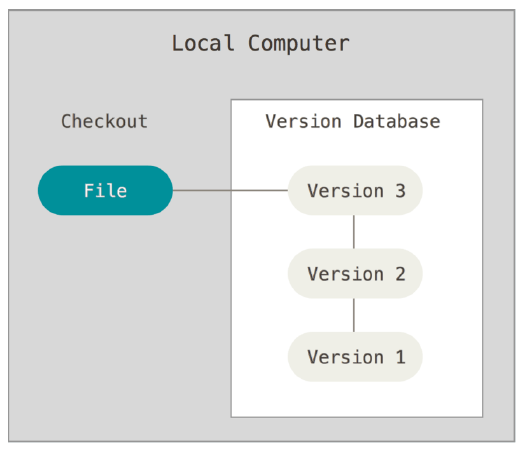
\includegraphics[scale=0.5]{LVC}  
	\caption[Local Version Control]{Local Version Control}
	\label{fig:LVC} 
\end{figure}

\textbf{\textit{Centralized Version Control System}}\\
CVCS(\textit{Centralized Version Control System}) memiliki sebuah \textit{server} yang menyimpan semua \textit{file} beserta historynya dan jumlah \textit{client} yang mengecek \textit{file} tersebut. Dengan adanya CVCS, semua orang mengetahui apa yang dilakukan oleh kolaborator yang mengerjakan proyek. Tetapi kelemahanya adalah ketika \textit{server} tersebut \textit{down}, tidak akan ada yang bisa berkolaborasi dan tidak dapat menyimpan perubahan yang sudah dikerjakan. Selain itu apabila data di \textit{server} tersebut hilang maka dan tidak melakukan \textit{back-up}, proyek yang sedang dikerjakan akan hilang beserta semua historinya. Struktur CVCS dapat dilihat pada Gambar~\ref{fig:CVCS}.

\begin{figure}[H]
	\centering  
	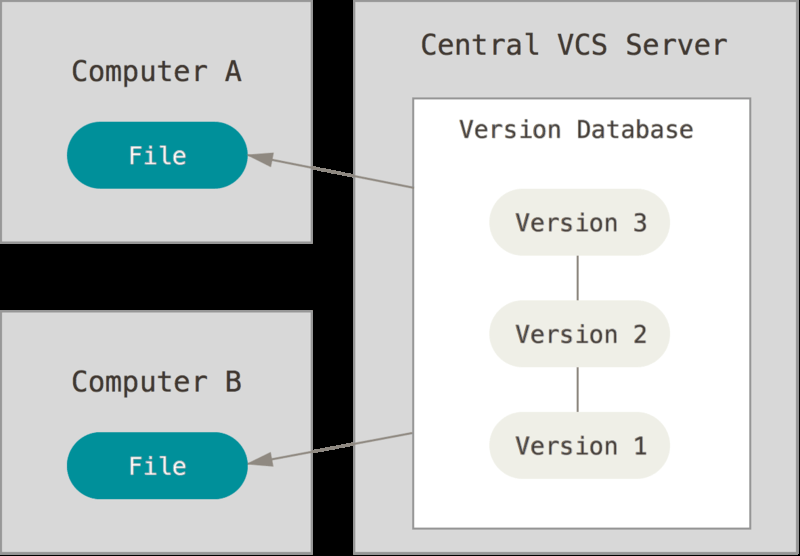
\includegraphics[scale=0.5]{CVCS}  
	\caption[Centralized Version Control]{Centralized Version Control}
	\label{fig:CVCS} 
\end{figure}

\textbf{\textit{Distributed Version Control System}}\\
Dalam DVCS(\textit{Distributed Version Control System}) seperti \textit{Git, Mercurial, Bazaar dan Darcs}, \textit{client} tidak mengecek versi terbaru dari \textit{file} tetapi \textit{client} menggandakan \textit{repository} termasuk historinya. Jika \textit{server} mati/kehilangan data, maka \textit{client} memiliki \textit{file back-up} untuk mengembalikanya.  Ilustrasi DVCS terdapat pada Gambar~\ref{fig:DVCS}.

\begin{figure}[H]
	\centering  
	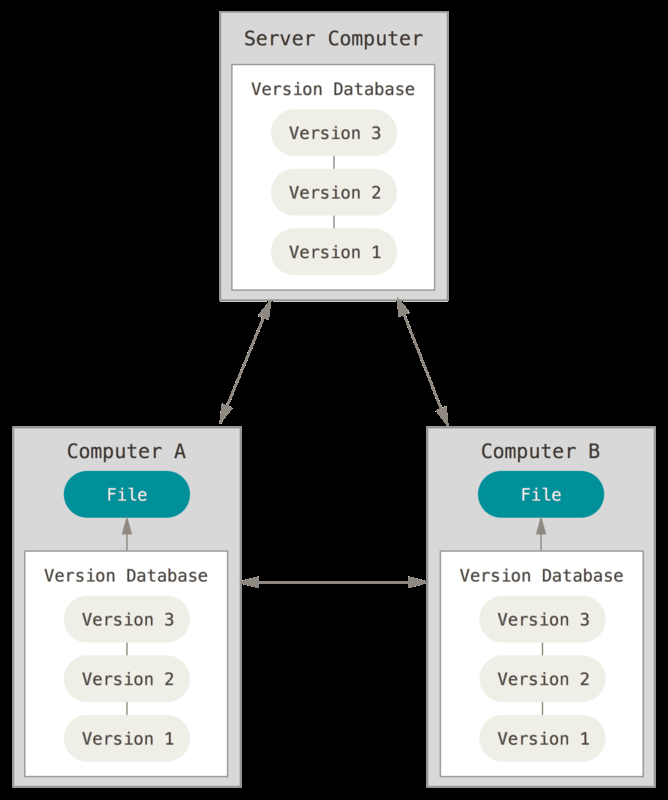
\includegraphics[scale=0.5]{DVCS}  
	\caption[Distributed Version Control]{Distributed Version Control}
	\label{fig:DVCS} 
\end{figure}

\textbf{\textit{Git}}\\
\textit{Git} merupakan sebuah \textit{version control} namun berbeda dengan VCS lainnya dilihat dari cara menyimpan datanya. Sistem seperti CVS, \textit{Subversion, Perforce, Bazzar} menyimpan data sebagai sekumpulan \textit{file} dan perubahan setiap \textit{file} disimpan setiap waktu. Pada \textit{Git}, data tersebut dianggap sebagai sekumpulan \textit{snapshot} dari \textit{miniature filesystem}. Setiap \textit{commit} atau menyimpan proyek, \textit{Git} seolah-olah mengambil gambar untuk melihat seperti apa \textit{file} yang terlihat pada saat itu dan menyimpannya sebagai referensi pada \textit{snapshot} tersebut. Singkatnya, apabila tidak ada \textit{file} yang diubah, Git tidak akan menyimpan \textit{file} lagi.\\

Hampir semua operasi pada \textit{Git} dapat dilakukan secara lokal. Ketika ingin menlihat histori suatu proyek, \textit{Git} akan mengambil data histori tersebut dari basis data lokal, sehingga tidak perlu memintanya ke \textit{server}. Selain itu, pengguna dapat bekerja secara \textit{offline}. Pada sistem lain seperti \textit{Perforce}, pengguna tidak dapat melakukan banyak hal jika tidak terkoneksi ke \textit{server} dan pada CVS, pengguna dapat mengubah \textit{file} tetapi tidak dapat \textit{commit} ke basis data. Pada \textit{Git}, pengguna dapat \textit{commit} dikarenakan \textit{Git} memiliki basis data lokal.\\

\textit{Git} memiliki 3 \textit{state} utama pada \textit{file} yaitu: 

\begin{itemize}
	\item \textit{committed} : data sudah tersimpan di basis data lokal.
	\item \textit{modified} : \textit{file} sudah diubah namun belum di\textit{commit} ke basis data.
	\item \textit{staged} : menandai file yang sudah dimodifikasi dalam versi sekarang untuk di\textit{commit}.
\end{itemize}

Terdapat 3 bagian utama dalam proyek \textit{Git} yaitu : 

\begin{itemize}
	\item \textit{Git directory} : tempat untuk menyimpan \textit{metadata} dan objek basis data untuk proyek yang dibuat. Ini adalah bagian terpenting dari \textit{Git} dan inilah yang di-\textit{copy} ketika \textit{clone repository} dari komputer lain.
	\item \textit{Working tree} : \textit{single checkout} sebuah versi dari proyek. \textit{File} diambil dari basis data yang sudah di\textit{compressed} di \textit{Git directory} dan disimpan pada \textit{disk} untuk digunakan dan dimodifikasi.
	\item \textit{Staging area} : sebuah \textit{file} yang ada di \textit{Git directory} yang menyimpan informasi tentang apa yang akan disimpan untuk \textit{commit} selanjutnya.  
\end{itemize}

Gambar~\ref{fig:gitState} di bawah ini menunjukan \textit{working tree, staging area dan Git directory}.

\begin{figure}[H]
	\centering  
	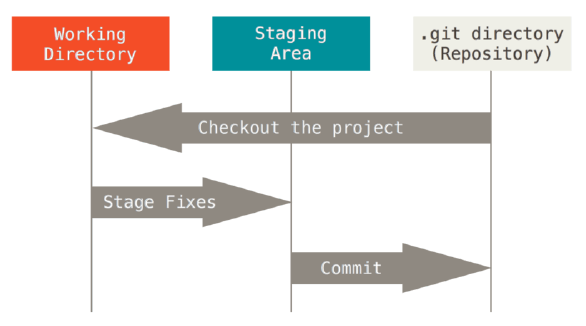
\includegraphics[scale=0.5]{gitState}  
	\caption[Working tree, staging area, dan Git directory]{Working tree, staging area, dan Git directory}
	\label{fig:gitState} 
\end{figure}

\textit{Workflow} pada \textit{Git} adalah sebagai berikut :

\begin{enumerate}
	\item Pengguna memodifikasi \textit{file} di \textit{working tree} milik pengguna.
	\item Pengguna memilih \textit{file} yang akan menjadi bagian dari \textit{commit} selanjutnya. \textit{File} yang terpilih akan ditambahkan ke \textit{staging area}. 
	\item Pengguna melakukan \textit{commit file} tersebut yang berada pada \textit{staging area} dan menyimpan \textit{snapshot} secara permanen ke \textit{Git directory}.
\end{enumerate}

Apabila versi tertentu dari sebuah \textit{file} sudah ada pada \textit{Git directory}, maka \textit{file} tersebut dalam berada dalam \textit{state committed}. Jika \textit{file} sudah dimodifikasi dan sudah ditambahkan ke \textit{staging area}, maka file tersebut dalam state \textit{staged}. Jika \textit{file} sudah diubah dan sudah di\textit{checkout} tetapi belum dalam \textit{state staged}, maka \textit{file} tersebut dalam \textit{state modified}.\\

Ada beberapa cara dalam menggunakan \textit{Git} yaitu dengan menggunakan \textit{command-line} dan beberapa GUI(\textit{Graphical User Interface}) yang memiliki kemampuan bermacam-macam. Pada umumnya digunakan \textit{command-line}, karena \textit{command-line} dapat menjalankan semua perintah \textit{Git} sedangkan GUI hanya memiliki sebagian fungsionalitas pada \textit{Git} supaya mudah digunakan.\\ 

\textbf{Mendapatkan \textit{Git Repository}}\\
Untuk mendapatkan \textit{Git repository} ada 2 cara yaitu : menjadikan sebuah proyek yang terdapat pada direktori lokal yang belum dalam \textit{version control} lalu menjadikannya sebagai \textit{Git repository} atau \textit{clone Git repository} yang sudah ada.\\

Jika memiliki direktori proyek yang belum dalam \textit{version control} dan ingin mengontrolnya menggunakan \textit{Git}, hal pertama yang harus dilakukan adalah dengan membuka direktori proyek. Perintah untuk membuat repository pada \textit{Windows} adalah dengan mengetikan perintah \textit{cd /c/user/my\_project} sesudah itu ketik perintah \textit{git init}. Perintah tersebut akan membuat subdirektori bernama \textit{.git} yang mengandung semua repository yang dibutuhkan. Setelah mengetikan perintah di atas, proyek tersebut belum di-\textit{track} sama sekali. Untuk men-\textit{track file-file} pada sebuah proyek, pertama gunakan perintah \textit{git add} untuk men-\textit{track file} yang diinginkan kemudian ketik \textit{git commit} untuk commit file tersebut.\\

\textit{Clone repository} adalah mendapatkan \textit{copy} dari \textit{repository} yang sudah ada. Perintah yang digunakan adalah \textit{git clone}. Tidak hanya \textit{file-file} pada \textit{repository} saja yang di\textit{copy}, tetapi semua histori pada \textit{repository} tersebut akan ikut ter\textit{copy}. Perintah \textit{git clone} diikuti dengan \textit{url}. \textit{Url} ini berisi \textit{link} di mana \textit{repository} berada.\\

\textbf{\textit{Record} Perubahan pada \textit{Repository}}\\
Setiap \textit{file} dalam direktori memiliki 2 \textit{state} yaitu \textit{tracked} atau \textit{untracked}. \textit{Tracked file} adalah \textit{file} yang berada pada \textit{snapshot} terakhir. \textit{Tracked file} adalah \textit{file} yang \textit{Git} ketahui sekarang. \textit{Untracked file} adalah \textit{file} yang tidak berada pada \textit{snapshot} terakhir. Ketika \textit{file} diubah, \textit{Git} melihat bahwa \textit{file} tersebut sudah dimodifikasi, karena \textit{file} tersebut diubah setelah \textit{commit} terakhir. Kemudian \textit{file} yang sudah dimodifikasi tersebut di-\textit{stage} dan \textit{commit} semua \textit{file} yang sudah di\textit{staged} tersebut. Gambar~\ref{fig:lifecycle} menunjukan siklus hidup dari status \textit{file}.

\begin{figure}[H]
	\centering  
	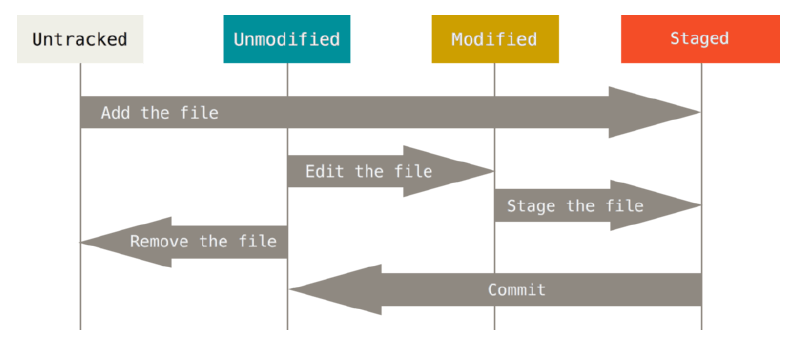
\includegraphics[scale=0.5]{lifecycle}  
	\caption[Siklus hidup pada status \textit{file}]{Siklus hidup pada status file}
	\label{fig:lifecycle} 
\end{figure}

Perintah \textit{git status} digunakan untuk mengecek status \textit{file}. Jika mengetik perintah sesudah \textit{clone}, maka tidak ada \textit{untracked file} karena pada saat \textit{clone}, tidak ada \textit{file} yang dimodifikasi. Bila menambahkan sebuah \textit{file} baru atau mengubah \textit{file} lalu mengetik perintah \textit{git status}, maka akan diberitahukan bahwa terdapat \textit{untracked file}. Karena itu untuk men-\textit{track file} baru, gunakan perintah \textit{git add} yang diikuti dengan nama \textit{file}nya seperti contoh ini : \textit{git add README}. Perintah \textit{git add} tidak hanya digunakan untuk men-\textit{track file} baru. Selain digunakan untuk men-\textit{track file}, perintah \textit{git add} digunakan untuk stage \textit{file} yang sudah dimodifikasi.\\

Tidak semua \textit{file} akan ditambahkan secara otomatis oleh \textit{Git} atau ada \textit{file} yang ditunjukan sebagai \textit{file untracked}. Hal ini dapat diatasi dengan membuat sebuah \textit{file} yang bernama \textit{.gitignore}. \textit{File .gitignore} ini berisi \textit{file-file} yang tidak akan di-\textit{track} oleh \textit{Git}. \textit{File} yang biasanya ada dalam \textit{.gitignore} adalah \textit{log}, \textit{tmp} atau \textit{file} dokumentasi yang di\textit{generate} secara otomatis. Adapun aturan untuk \textit{pattern} yang dapat dimasukan pada \textit{file .gitignore} diantaranya adalah :

\begin{itemize}
	\item Baris kosong atau baris yang diawali dengan tanda pagar(\#) akan dibiarkan.
	\item \textit{Standard glob patterns}.
	\item \textit{Pattern} diawali dengan garis miring(/) untuk mencegah rekusrif.
	\item \textit{Pattern} diakhiri dengan garis miring untuk menspesifikasikan direktori.
	\item Menegasikan \textit{pattern} diawali dengan tanda seru(!).
\end{itemize}

\textit{Glob pattern} adalah \textit{regular expression} yang digunakan oleh \textit{shells}. Tanda bintang(*) untuk nol atau beberapa karakter, [abc] untuk karakter apa saja yang berada di dalam kurung siku, tanda tanya(?) untuk sebuah karakter apa saja dan tanda kurung siku dengan tanda strip(-) untuk karakter antara sebuah karakter dengan karakter lainya.\\

Perintah \textit{git commit} digunakan untuk \textit{commit file} yang sudah diubah dan ditambahkan. \textit{File} tersebut harus sudah di-\textit{stage} dengan menggunakan perintah \textit{git add}. \textit{File} yang belum di-\textit{stage} akan berada dalam state \textit{modified} meskipun sudah melakukan \textit{commit}. Untuk menambahkan keterangan tentang \textit{file} yang di\textit{commit} dapat dituliskan perintah \textit{git commit -m} yang diikuti dengan keterangan yang ingin disampaikan. \\

\textbf{\textit{Git Branching}}\\
\textit{Branching} artinya membuat dan mengerjakan sebuah proyek di tempat yang berbeda namun masih dalam repository yang sama sehingga tidak mengubah proyek utama. Ketika \textit{commit}, \textit{Git} menyimpan objek \textit{commit} yang memiliki sebuah \textit{pointer} pada \textit{snapshot} sebuah konten yang sudah dalam \textit{state staged}. Objek ini mengandung nama pembuat dan alamat email, pesan yang diketik, dan \textit{pointer} ke \textit{commit}. \\

Misalkan seorang pengguna memiliki 3 \textit{file}, kemudian file tersebut semuanya di-\textit{stage} dan \textit{commit}. \textit{Staging file} akan mengkomputasi \textit{checksum} untuk setiap \textit{file}, menyimpan versi tersebut pada \textit{Git repository}(hal ini dapat disebut juga sebagai \textit{blobs}), dan menambah \textit{checksum} tersebut ke \textit{staging area}. Lalu \textit{Git} melakukan \textit{checksum} pada setiap \textit{subdirectory} dan menyimpan ketiga objek tersebut pada \textit{Git repository}. Sesudah itu \textit{Git} akan membuat objek \textit{commit} yang mengandung \textit{metadata} dan \textit{pointer} ke proyek \textit{root} sehingga dapat melihat \textit{snapshot} tersebut pada setiap versi. Sekarang, \textit{Git repository} memiliki 5 objek yaitu 3 \textit{blob} yang merepresentasikan 3 file, sebuah \textit{tree} yang mengandung isi direktori dan memberi nama \textit{blob} berdasarkan nama file yang di\textit{commit}, dan sebuah \textit{commit} dengan \textit{pointer} ke \textit{root tree} dan semua \textit{commit metadata}. Gambar~\ref{fig:branch} merupakan \textit{tree} dari penjelasan tersebut.

\begin{figure}[H]
	\centering  
	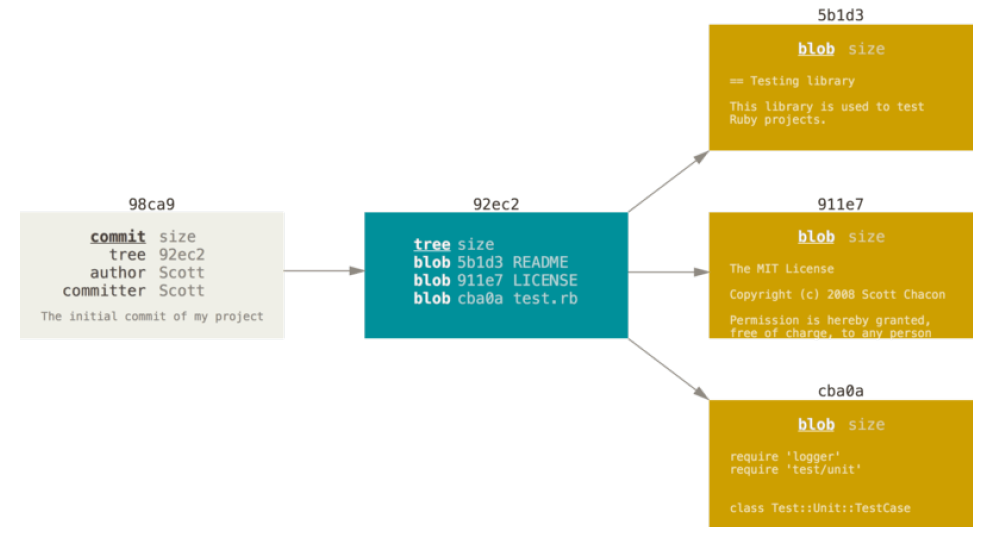
\includegraphics[scale=0.5]{branch}  
	\caption[Commit dan tree dari file yang dicommit]{Commit dan tree dari file yang dicommit}
	\label{fig:branch} 
\end{figure}

Jika ada perubahan pada proyek dan \textit{commit} proyek tersebut, maka \textit{commit} sesudahnya menyimpan \textit{pointer} pada \textit{commit} sebelum \textit{commit} terbaru seperti yang terdapat pada Gambar~\ref{fig:commitTree}. Jadi \textit{parent} dari sebuah \textit{commit} adalah \textit{commit} sebelumnya dan kemudian seterusnya.

\begin{figure}[H]
	\centering  
	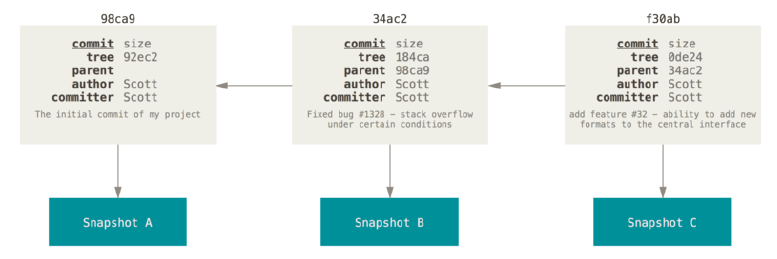
\includegraphics[scale=0.7]{commitTree}  
	\caption[Commit dan parent dari commit]{Commit dan parent dari commit}
	\label{fig:commitTree} 
\end{figure}

Nama \textit{branch} pada \textit{Git} awalnya disebut \textit{master}. Ketika \textit{commit}, pengguna diberikan \textit{branch master} yang menunjuk pada \textit{file} yang di\textit{commit} terakhir. Setiap \textit{commit}, pointer pada \textit{branch master} akan terus maju secara otomatis.\\ 

Untuk membuat branch baru, gunakan perintah \textit{git branch} diikuti dengan nama \textit{branch}. \textit{Git} menggunakan \textit{pointer} yang disebut dengan \textit{HEAD} untuk mengetahui bahwa pengguna sedang berada dalam \textit{branch} tertentu. Bila membuat \textit{branch} baru, posisi \textit{HEAD} tetap berada pada \textit{branch} yang sekarang. Perintah \textit{git branch} hanya membuat \textit{branch} baru dan tidak berpindah ke \textit{branch} yang baru saja dibuat. Pada Gambar~\ref{fig:head}, jika mengetikan perintah \textit{git branch testing}, \textit{branch testing} akan dibuat tetapi \textit{pointer HEAD} akan tetap berada pada \textit{branch master}.

\begin{figure}[H]
	\centering  
	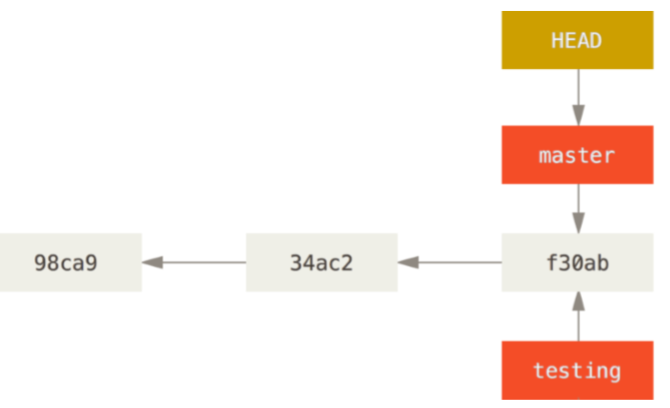
\includegraphics[scale=0.5]{head}  
	\caption[\textit{Pointer HEAD} menunjuk \textit{branch master}]{\textit{Pointer HEAD} menunjuk \textit{branch master}}
	\label{fig:head} 
\end{figure}

Untuk pindah \textit{branch}, gunakan perintah \textit{git checkout} diikuti dengan nama \textit{branch}. \textit{Pointer HEAD} akan berpindah ke \textit{branch} tersebut. Bila pada \textit{branch} tersebut pengguna melakukan \textit{commit}, maka \textit{branch} tersebut akan maju beserta dengan \textit{pointer HEAD} seperti dicontohkan pada Gambar~\ref{fig:changeHead}. Misalkan pengguna \textit{commit} pada \textit{branch testing}, maka hanya \textit{branch testing} saja yang maju sedangkan \textit{branch master} tidak. Ini dikarenakan \textit{file} pada \textit{branch master} tidak diubah.\\

\begin{figure}[H]
	\centering  
	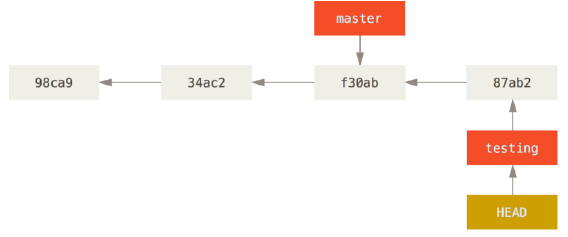
\includegraphics[scale=0.7]{changeHead}  
	\caption[\textit{Pointer HEAD} beserta \textit{branch testing}]{\textit{Pointer HEAD} beserta \textit{branch testing}}
	\label{fig:changeHead} 
\end{figure}

Perintah \textit{git checkout} tidak hanya sebatas untuk pindah ke \textit{branch} yang diinginkan. \textit{File} yang ada pada \textit{working directory} akan diubah dengan \textit{file} yang ada pada \textit{branch} tersebut. Bila berpindah ke \textit{branch} sebelumnya, maka \textit{file} dalam \textit{working directory} akan dikembalikan sesuai dengan \textit{commit} terakhir dari \textit{branch} tersebut. Untuk membuat \textit{branch} baru sekaligus pindah \textit{branch}, gunakan perintah \textit{git checkout -b} diikuti dengan nama \textit{branch} yang ingin dibuat. Dengan ini \textit{pointer HEAD} akan berada pada \textit{branch} yang baru dibuat. \\

\textbf{\textit{Basic Merging}}\\
\textit{Merging} adalah penggabungan sebuah \textit{branch} dengan \textit{branch} lain. Perntah untuk \textit{merge} adalah \textit{git merge} diikuti dengan nama \textit{branch} yang ingin digabungkan. Bila sebuah \textit{branch} ingin digabungkan dengan \textit{branch} yang memiliki \textit{direct ancestor} yang berbeda, \textit{Git} akan melakukan \textit{three way merge}. \textit{Three way merge} ini menggunakan 2 \textit{snapshot} yang menunjuk pada \textit{branch} yang akan digabungkan dan 1 \textit{snapshot} yang menunjuk pada \textit{ancestor} yang sama dari kedua \textit{branch} tersebut seperti yang terdapat pada Gambar~\ref{fig:threeWayMerge}. Kemudian \textit{Git} membuat \textit{snapshot} baru yang merupakan hasil dari \textit{three way merge} dan secara otomatis akan membuat \textit{commit} yang baru seperti yang terlihat pada Gambar~\ref{fig:mergeCommit}. Hal ini disebut sebagai \textit{merge commit} karena memiliki lebih dari 2 \textit{parent}.

\begin{figure}[H]
	\centering  
	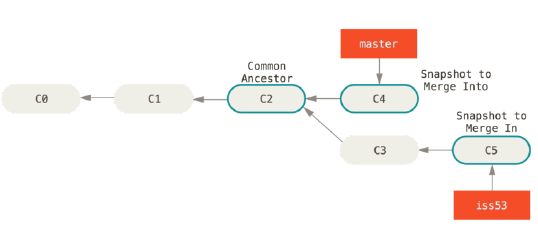
\includegraphics[scale=0.7]{threeWayMerge}  
	\caption[3 \textit{snapshot} yang digunakan dalam \textit{three way merge}]{3 \textit{snapshot} yang digunakan dalam \textit{three way merge}}
	\label{fig:threeWayMerge} 
\end{figure}

\begin{figure}[H]
	\centering  
	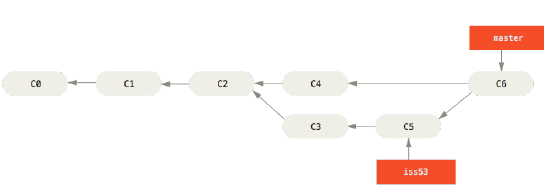
\includegraphics[scale=0.7]{mergeCommit}  
	\caption[\textit{Merge commit}]{\textit{Merge commit}}
	\label{fig:mergeCommit} 
\end{figure}

\textit{Merge} pada \textit{Git} mungkin akan menimbulkan konflik. Hal ini dapat terjadi apabila \textit{file} yang sama pada kedua \textit{branch} tersebut diubah pada bagian yang sama. Ketika mengetikan perintah \textit{git merge}, maka \textit{Git} tidak akan membuat \textit{merge commit} secara otomatis. Proses \textit{merge} akan dijeda sesudah konflik tersebut sudah diselesaikan. Untuk menangani konflik tersebut, pilihlah salah satu \textit{branch}. Maksdud dari memilih salah satu \textit{branch} adalah dengan mengubah \textit{file} yang berada pada salah satu \textit{branch}. Sesudah mengubah \textit{file} pada branch yang dipilih, maka \textit{Git} akan \textit{merge branch} jika tidak ada konflik lagi.

\textbf{\textit{Remote Branches}}\\
\textit{Remote-tracking branches} adalah referensi dari \textit{state remote branches}. Referensi tersebut merupakan referensi lokal yang hanya dapat dipindahkan oleh \textit{Git} untuk memastikan jika referensi tersebut merepresentasikan \textit{state} dari \textit{remote repository}. \textit{<remote>/<branches>} merupakan \textit{remote-tracking branches}. Jika ingin mengecek \textit{file} pada \textit{branch master} yang berada dalam \textit{remote origin}, maka pengguna harus mengecek \textit{branch origin/master}. Sama seperti \textit{branch master}, \textit{origin} juga merupakan penamaan \textit{remote} secara otomatis ketika \textit{clone repository}. Jika pengguna mengubah \textit{branch} lokal maka \textit{branch} milik server tidak akan berubah dan hanya \textit{pointer} pada lokal saja yang berubah. Maka dari itu \textit{branch} di lokal dan \textit{branch} di \textit{server} bisa saja berbeda seperti yang terlihat pada Gambar~\ref{fig:diverge}. Untuk mensinkron \textit{branch} di lokal dan \textit{branch} di \textit{server}, gunakan peirntah \textit{git fetch} diikuti dengan nama \textit{remote}. Dengan cara ini, beberapa data yang belum dimiliki akan diambil dari \textit{server}, meng-\textit{update} basis data lokal dan memindahkan \textit{pointer} ke posisi yang terbaru seperti yang terlihat pada Gambar~\ref{fig:fetch}.\\

\begin{figure}[H]
	\centering  
	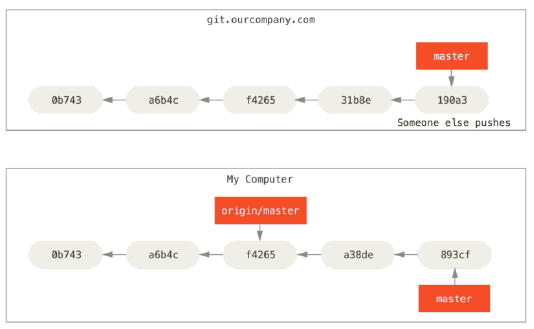
\includegraphics[scale=0.7]{diverge}  
	\caption[Perbedaan pada \textit{branch} lokal dan \textit{remote}]{Perbedaan pada \textit{branch} lokal dan \textit{remote}}
	\label{fig:diverge} 
\end{figure}

\begin{figure}[H]
	\centering  
	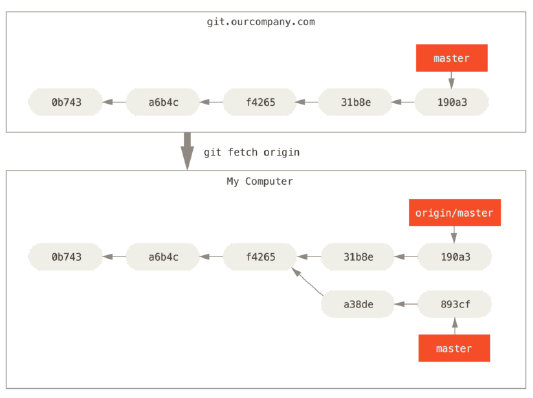
\includegraphics[scale=0.7]{fetch}  
	\caption[\textit{Update remote-tracking branches} menggunakan perintah \textit{git fetch}]{\textit{Update remote-tracking branches} menggunakan perintah \textit{git fetch}}
	\label{fig:fetch} 
\end{figure}

Jika ingin membagikan \textit{branch} ke pengguna lain, pengguna harus \textit{push branch} tersebut ke \textit{remote} karena \textit{branch} lokal tidak sinkron secara otomatis dengan \textit{remote}. Perintah yang digunakan untuk \textit{push} adalah \textit{git push} diikuti dengan nama \textit{remote} dan nama \textit{branch}.\\ 

\textit{Check out branch} lokal dari \textit{remote-tracking branch} secara otomatis akan membuat \textit{tracking branch}. \textit{Tracking branch} adalah \textit{branch} lokal yang memiliki hubungan langsung dengan \textit{branch remote}. Jika berada pada \textit{tracking branch} dan mengetikan perintah \textit{git pull}, secara otomatis \textit{Git} mengetahui \textit{server} mana yang akan di-\textit{fetch} dan \textit{branch} apa yang akan di-\textit{merge}. Bila \textit{clone repository}, maka secara otomatis akan membuat sebuah \textit{branch} yang bernama master yang men-\textit{track origin/master}. Untuk mengatur \textit{tracking branch}, perintah yang digunakan adalah \textit{git checkout -b <branch> <remote>/<branch>}. \textit{Git} menyediakan perintah \textit{git checkout --track <remote>/<branch>} sebagai shortcut dari perintah checkout sebelumnya. Perintah \textit{git checkout} juga dapat digunakan untuk mengatur \textit{branch} lokal dengan nama yang berbeda dari \textit{branch remote}. Jika sudah memiliki \textit{branch} lokal dan ingin mengatur \textit{branch} tersebut ke \textit{branch remote} yang sudah di-\textit{pull}, gunakan opsi \textit{-u} atau \textit{--set-upstream-to} pada perintah \textit{git branch}. Untuk melihat \textit{tracking branch} yang sudah diatur, gunakan opsi \textit{-vv} pada perintah \textit{git branch}. Perintah ini akan menampilkan \textit{list} dari \textit{branch} lokal dengan informasi tambahan mengenai \textit{tracking} pada setiap \textit{branch} dan apakah \textit{branch} lokal tersebut memiliki \textit{ahead, behind} atau keduanya. \textit{Ahead} adalah ada \textit{commit} lokal yang belum di-\textit{push} ke \textit{server}, sedangkan \textit{behind} adalah \textit{commit} yang belum digabungkan. Perintah ini tidak langsung mengambil datanya dari \textit{server} tetapi data tersebut merupakan data saat terakhir \textit{fetch} dari \textit{server}. Untuk mendapatkan data yang terbaru, harus \textit{fetch} dari semua \textit{remote} kemudian mengetikan perintah \textit{git branch -vv}.\\

\textit{Perintah git fetch} akan mengambil semua perubahan yang ada pada \textit{server} yang tidak dimiliki oleh \textit{branch lokal}, tetapi tidak mengubah \textit{working directory} yang sesuai dengan \textit{branch remote}. Perintah \textit{git pull} digunakan untuk mengubah \textit{working directory}. Perintah ini akan melihat \textit{server} dan \textit{branch} yang sedang di-\textit{track}, mengambil data dari \textit{server} tersebut dan menggabungkanya. Singkatnya, perintah \textit{git pull} merupakan gabungan dari perintah \textit{git fetch} dengan \textit{git merge}.\\

\textit{Branch} pada \textit{remote} dapat dihapus dengan menggunakan opsi \textit{--delete} pada perintah \textit{git push}. \textit{Branch} pada \textit{remote} tidak sepenuhnya dihapus, tetapi hanya \textit{pointer}nya saja yang dihilangkan. Jika \textit{branch} tidak sengaja terhapus, maka data pada branch dapat dikembalikan/di\textit{back-up}.\\

\textbf{\textit{Rebasing}}\\
Selain \textit{merge}, ada cara lain untuk menggabungkan kedua \textit{branch} yaitu \textit{rebasing}. Cara kerja dari \textit{rebasing} adalah mencari \textit{ancestor} yang sama dari kedua \textit{branch}, mendapatkan perbedaan setiap \textit{commit} pada \textit{branch} saat ini, menyimpan perbedaan tersebut pada \textit{file} sementara, mengatur ulang \textit{branch} ke \textit{commit} yang sama dengan \textit{branch} yang akan di\textit{rebase}, dan menerapkan setiap perubahannya. Contoh \textit{rebasing} dapat dilihat pada Gambar~\ref{fig:rebasing}. \textit{Commit} C4 pada \textit{branch experiment} berpindah dari C4 ke C4' yang berada di atas C3. Setelah \textit{rebasing}, \textit{merge} kedua \textit{branch} tersebut sehingga hasilnya terlihat seperti pada Gambar~\ref{fig:rebasingMerge}. Untuk \textit{rebasing}, gunakan perintah \textit{git rebase} kemudian diikuti nama \textit{branch} yang ingin di\textit{rebase}. 

\begin{figure}[H]
	\centering  
	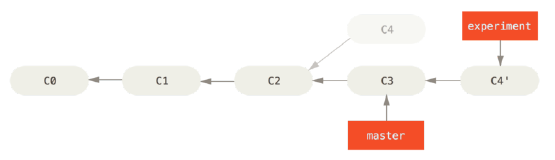
\includegraphics[scale=0.8]{rebasing}  
	\caption[\textit{Rebasing commit} C4 ke C3]{\textit{Rebasing commit} C4 ke C3}
	\label{fig:rebasing} 
\end{figure}

\begin{figure}[H]
	\centering  
	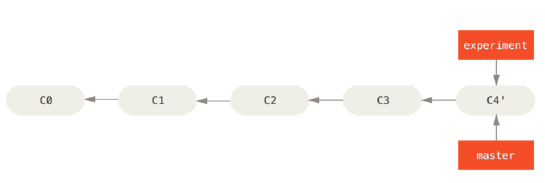
\includegraphics[scale=0.8]{rebasingMerge}  
	\caption[\textit{Merge branch} setelah \textit{rebasing}]{\textit{Merge branch} setelah \textit{rebasing}}
	\label{fig:rebasingMerge} 
\end{figure}

Hasil terakhirnya tidak berbeda dengan menggunakan perintah \textit{merge}, namun \textit{rebasing} membuat histori menjadi lebih sedikit dibandingkan dengan \textit{merge}. \textit{Rebasing} juga berguna dalam berkontribusi pada proyek yang bukan milik sendiri. Hal ini akan mempermudah kerja pemilik proyek, karena pemilik proyek hanya tinggal \textit{clean apply} saja. \\

\textbf{\textit{GitHub}}\\
\textit{GitHub} merupakan \textit{single host} terbesar untuk \textit{Git repository} dan sebagai titik tengah dari kolaborasi untuk jutaan pengembang dan proyek. Persentase terbesar dari semua \textit{Git repository} di\textit{hosting} di \textit{GitHub} dan banyak proyek \textit{open-source} menggunakanya untuk \textit{Git hosting, code review, issue tracking} dan lainnya. \\

\textbf{\textit{Fork}}\\
Jika pengguna ingin berkontribusi pada proyek yang sudah ada dan pengguna tidak memiliki akses untuk \textit{push}, maka pengguna dapat \textit{fork} proyek tersebut. Ketika proyek tersebut telah di-\textit{fork}, \textit{GitHub} akan membuatkan sebuah \textit{copy/clone} dari proyek tersebut yang sekarang sudah menjadi milik penggunanya dan dapat di\textit{push}. Orang lain dapat \textit{fork} proyek, \textit{push} proyek, dan berkontribusi dalam perubahan tersebut dan menyarankan untuk menggabungkan perubahan tersebut dengan \textit{repository} aslinya dengan membuat \textit{Pull Request}.\\


Berikut adalah langkah-langkah untuk berkolaborasi dalam GitHub: 

\begin{enumerate}
	\item \textit{Fork} proyek yang diinginkan.
	\item Buat topik \textit{branch} dari \textit{master}.
	\item Lakukan \textit{commit} untuk memperbaiki proyek.
	\item \textit{Push branch} ke proyek \textit{GitHub}.
	\item Buka \textit{Pull Request} di \textit{GitHub}.
	\item Diskusikan dan \textit{commit} proyek tersebut apabila proyek tersebut masih membutuhkan perbaikan.
	\item Pemilik proyek \textit{merges}/menggabungkan atau menutup \textit{Pull Request}.\\
\end{enumerate}

\textbf{\textit{Pull Request}}\\
\textit{Pull Request} membuka tempat diskusi untuk \textit{owner(pemilik repository)} dan kontributor sehingga dapat berkomunikasi tentang perubahan tersebut sampai \textit{owner} merasa puas dan senang. Setelah itu \textit{owner} akan \textit{merge}/menggabungkan perubahan tersebut. Setelah kontributor sudah membuat \textit{Pull Request}, pemilik proyek dapat melihat saran perubahan proyek dari orang lain dan memberikan komentar/keterangan pada perubahan tersebut. Pemilik proyek dapat melihat perbedaan pada kode pemilik proyek dengan perubahan yang disarankan tersebut dan pemilik proyek dapat mengomentari baris pada kode tersebut. Orang lain dapat memberikan komentar pada \textit{Pull Request}. Sesudah pemilik proyek memberikan keterangan tentang perubahan tersebut, kontributor menjadi tahu apa yang harus dilakukan agar perubahan tersebut dapat disetujui. Apabila perubahan tersebut membuat pemilik proyek puas, pemilik proyek akan \textit{merge} perubahan tersebut dengan proyek aslinya dan otomatis akan menutup \textit{Pull Request}.	

\end{itemize}
		
		\item \textbf{Melakukan analisis dan menentukan objek-objek pada Snake 360}\\
		{\bf Status :} Ada sejak rencana kerja skripsi.\\
		{\bf Hasil :} 

\begin{itemize}		
\item \textbf{Analisis Permainan \textit{Snake} yang Sudah Ada}\\
Permainan \textit{Snake} yang akan dianalisis adalah \textit{Slither.io}. \textit{Slither.io} adalah permainan \textit{web} yang dapat dimainkan oleh lebih dari 1 pemain(\textit{multiplayer}). Cara bermainya mirip seperti permainan \textit{Snake} pada umumnya yaitu ular harus memakan makanan untuk mendapatkan skor. Dalam permainan ini, setiap pemain berkompetisi untuk menjadi pemain terbaik dengan cara mendapatkan skor sebanyak-banyaknya. Pemain akan kalah apabila ular milik pemain menabrak ular milik pemain lain.\\

\textbf{Ular dan Makanan}\\
Ular pada \textit{Slither.io} dibentuk dengan menggunakan sekumpulan lingkaran yang saling berdempetan satu sama lain seperti pada Gambar~\ref{fig:slitherUlar}. Bagian kepala pada ular ditandai menggunakan sepasang mata. Ketika memakan makanan, tubuh ular akan memanjang dengan menambahkan sebuah lingkaran pada bagian ekor ular. Setiap memulai permainan, tubuh ular akan memiliki warna yang ditentukan secara acak.

Makanan pada \textit{Slither.io} berbentuk lingkaran. Makanan ini ada yang berukuran besar dan ada yang berukuran kecil. Makanan ini tersebar pada labirin, jumlahnya sangat banyak dan warnanya bermacam-macam. Gambar~\ref{fig:slitherMakanan} merupakan sekumpulan makanan yang terdapat pada labirin. Setiap makanan akan menambah skor sebanyak 1 poin.

\begin{figure}[H]
	\centering
	\begin{minipage}{.5\textwidth}
		\caption[Ular pada \textit{Silther.io}]{Ular pada \textit{Silther.io}}
		\centering
		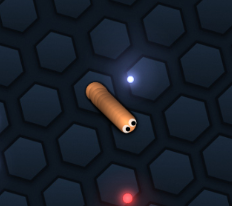
\includegraphics[scale=0.7]{slitherUlar}
		\label{fig:slitherUlar} 
	\end{minipage}%
	\begin{minipage}{.5\textwidth}
		\caption[Makanan pada \textit{Slither.io}]{Makanan pada \textit{Slither.io}}
		\centering
		
\includegraphics[scale=0.7]{slitherMakanan}
		\label{fig:slitherMakanan} 
	\end{minipage}
\end{figure}

\textbf{Pergerakan Ular}\\
Ular pada \textit{Slither.io} digerakan dengan menggunakan keyboard dan \textit{mouse}. Tombol ke kiri akan membuat ular bergerak berlawanan arah jarum jam dan tombol ke kanan akan membuat ular bergerak searah jarum jam. Semakin lama tombol ditekan, maka ular akan berbelok lebih cepat. Kursor pada \textit{mouse} membuat ular bergerak ke arah posisi kursor tersebut. Ular dapat melaju dengan cepat(\textit{speed up}) dengan menekan tombol \textit{mouse} kiri seperti yang terdapat pada Gambar~\ref{fig:slitherSpeed}. Ketika ular sedang melaju dengan cepat, total skor yang didapat akan berkurang. 

\begin{figure}[H]
	\centering  
	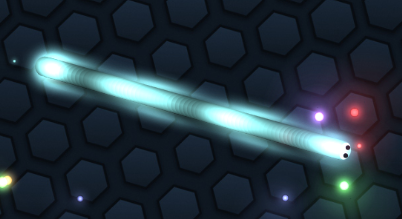
\includegraphics[scale=0.7]{slitherSpeed}  
	\caption[Ular sedang melaju dengan cepat(\textit{speed up})]{Ular sedang melaju dengan cepat(\textit{speed up})}
	\label{fig:slitherSpeed} 
\end{figure}

\textbf{Labirin}\\
Labirin pada \textit{Slither.io} hanya ada 1 saja. Labirin ini berbentuk lingkaran yang sisinya dikelilingi oleh dinding. Apabila ular menabrak dinding labirin, maka permainan akan berakhir. Labirin ini cukup besar sehingga sangat kecil kemungkinan ular untuk menabrak dinding labirin. Gambar~\ref{fig:slitherLabirin} menunjukan peta labirin pada \textit{Slither.io}. Pada peta labirin tersebut terdapat sekumpulan titik bewarna abu-abu yang merepresentasikan makanan.

\begin{figure}[H]
	\centering  
	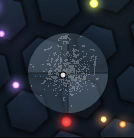
\includegraphics[scale=1]{slitherLabirin}  
	\caption[Peta labirin pada \textit{Slither.io}]{Peta labirin pada \textit{Slither.io}}
	\label{fig:slitherLabirin} 
\end{figure}

\item \textbf{Analisis Sistem yang Dibangun}\\
Permainan \textit{Snake} 360 yang akan dibangun memiliki cara bermain yang mirip seperti permainan Snake pada umumnya. Perbedaan antara \textit{Snake} 360 dengan permainan \textit{Snake} pada umumnya adalah \textit{Snake} 360 dapat menambahkan level dan labirin sendiri. 

\textbf{Menggambar Ular dan Apel}\\
Tubuh ular dibuat menggunakan sekumpulan \textit{line}/garis pendek. Setiap bagian tubuh ular memiliki panjang sebesar 1 \textit{pixel} dan lebar tubuhnya sebesar 5 \textit{pixel}. Bagian tubuh ular dibuat pendek untuk memudahkan pengecekan jika terjadi ular menabrak tubuhnya sendiri. Untuk lebar ular, disesuaikan dengan besar apel yaitu 10 \textit{pixel}. Setiap bagian tubuh ular memiliki koordinat masing-masing. Koordinat setiap bagian tubuh disimpan pada sebuah \textit{array} agar menggambar ular menjadi lebih mudah. Dalam tahap ini, tubuh ular masih berupa sekumpulan titik-titik yang merupakan koordinat bagian tubuh ular seperti pada Gambar~\ref{fig:titikUlar}. Algoritma untuk menggambar ular adalah dengan mengambil koordinat bagian tubuh ular mulai dari elemen \textit{array} paling pertama(arr[0]) dan elemen \textit{array} selanjutnya(arr[1]) lalu buat garis yang \textit{start point}nya adalah elemen pertama(arr[0]) dan \textit{end point}nya adalah elemen \textit{array} kedua(arr[1]). Setelah itu ambil koordinat elemen \textit{array} yang merupakan \textit{end point} pada garis sebelumnya(arr[1]) dengan elemen \textit{array} selanjutnya(arr[2]) dan gambar garisnya. Lakukan hal tersebut sampai \textit{end point} garis mencapai elemen \textit{array} paling akhir. Setelah digambar maka ular akan terlihat seperti Gambar~\ref{fig:garisUlar}.

\begin{figure}[H]
	\centering
	\begin{minipage}{.45\textwidth}
		\caption[Koordinat bagian tubuh ular pada \textit{array}]{Koordinat bagian tubuh ular pada \textit{array}}
		\centering
		\captionsetup{width=.3\textwidth}
		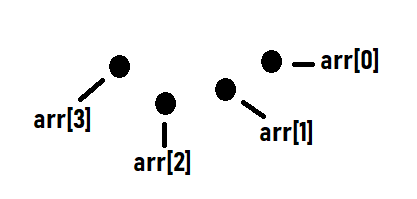
\includegraphics[scale=0.55]{titikUlar}
		\label{fig:titikUlar} 
	\end{minipage}%
	\hfill
	\begin{minipage}{.45\textwidth}
		\caption[Tubuh ular setelah digambar menggunakan garis]{Tubuh ular setelah digambar menggunakan garis}
		\centering
		\captionsetup{width=.3\textwidth}
		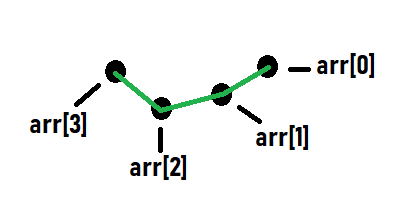
\includegraphics[scale=0.55]{garisUlar}
		\label{fig:garisUlar} 
	\end{minipage}
\end{figure}

Untuk membuat apel digunakan \textit{quadratic B\'ezier curve}. Kurva ini digunakan untuk membuat bagian-bagian apel yang melengkung. Bagian tersebut ditandai dengan lingkaran bewarna merah seperti yang ditunjukan pada Gambar~\ref{fig:apel}(gambar diambil dari pinterest:https://www.pinterest.com/pin/ 690317449105509454)

\begin{figure}[H]
	\centering  
	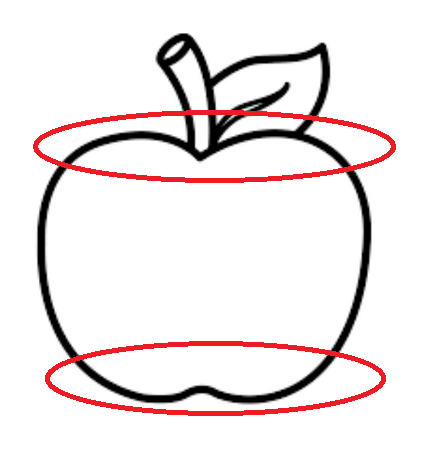
\includegraphics[scale=0.5]{apel}  
	\caption[Bagian pada apel(lingkaran merah) yang akan dibuat menggunakan kurva]{Bagian pada apel(lingkaran merah) yang akan dibuat menggunakan kurva}
	\label{fig:apel} 
\end{figure}

Pertama, tentukan besar apel yang ingin dibuat. Dalam permainan ini besar apel yang dibuat adalah 10 pixel. Besar apel dibuat lebih besar dari lebar ular karena jika besar apel sama dengan lebar ular, besar apel terlihat sangat kecil. Selain itu, apel ini digambar pada layout yang berbentuk persegi. Layout persegi ini juga dapat mempermudah penggambaran apel. Karena menggunakan layout persegi, maka origin terletak pada titik sudut di sebelah kiri atas. Setelah itu, gambar setiap bagian apel. Bagian apel dibagi menjadi 4 seperti pada Gambar~\ref{fig:apel2} sehingga besar setiap bagian apel tersebut adalah 5 pixel. 

\begin{figure}[H]
	\centering  
	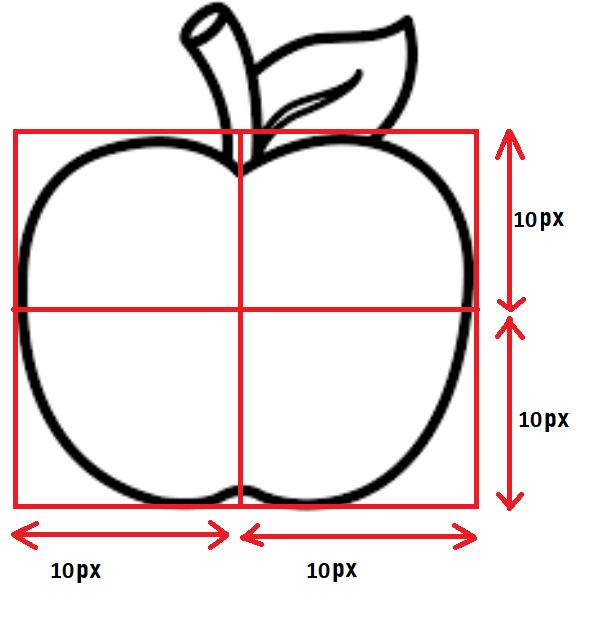
\includegraphics[scale=0.4]{apel2}  
	\caption[Pembagian gambar apel dengan layout persegi beserta ukuran pada setiap bagian]{Pembagian gambar apel dengan layout persegi beserta ukuran pada setiap bagian}
	\label{fig:apel2} 
\end{figure}

Gambar bagian atas apel terlebih dahulu. Gunakan method moveTo() untuk menentukan titik mulainya. Titik mulainya terletak pada bagian tengah atas apel yang melengkung ke dalam. Dari titik itu, buat kurva yang control pointnya adalah titik ujung layout persegi. Jika ingin menggambar bagian kiri apel terlebih dahulu maka control pointnya adalah titik ujung kiri layout tersebut. Setelah itu, tentukan end point kurva tersebut. Pada Gambar~\ref{fig:apel3} terdapat start point, control point dan end point untuk membuat bagian sisi kiri atas apel. Sesudah itu, buatlah bagian bawah apel. Caranya sama seperti sebelumnya namun control pointnya dan end pointnya berbeda. Posisi control pointnya sedikit menjorok ke dalam dan posisi end pointnya terdapat di tengah bawah seperti pada Gambar~\ref{fig:apel4}. Start point tidak perlu diatur lagi, karena start pointnya sudah tergantikan dengan posisi end point pada kurva sebelumnya. Sampai pada bagian ini, bagian kiri apel sudah selesai dibuat. Untuk membuat bagian kanan apel, caranya sama seperti membuat bagian kiri apel. Karena bagian kiri apel simetris dengan bagian kanan apel, maka hanya perlu mengubah control point dan end pointnya saja. Dengan memanfaatkan bentuk simetris dari apel, maka jarak antara control point dan end point pada bagian kiri apel dengan batasan tengah sama dengan jarak antara control point dan end point dengan batas tengah pada bagian kanan apel. 

\begin{figure}[H]
	\centering
	\begin{minipage}{.45\textwidth}
		\caption{Start point, control point dan end point untuk menggambar apel bagian kiri atas}
		\centering
		\captionsetup{width=.3\textwidth}
		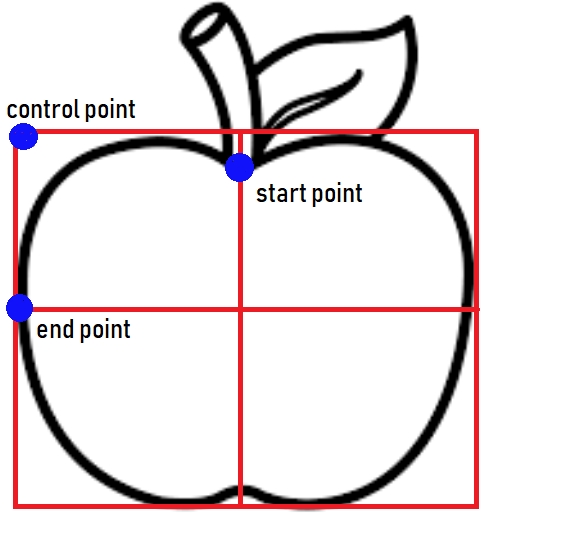
\includegraphics[scale=0.38]{apel3}
		\label{fig:apel3} 
	\end{minipage}%
	\hfill
	\begin{minipage}{.45\textwidth}
		\caption{Start point, control point dan end point untuk menggambar apel bagian kiri bawah}
		\centering
		\captionsetup{width=.3\textwidth}
		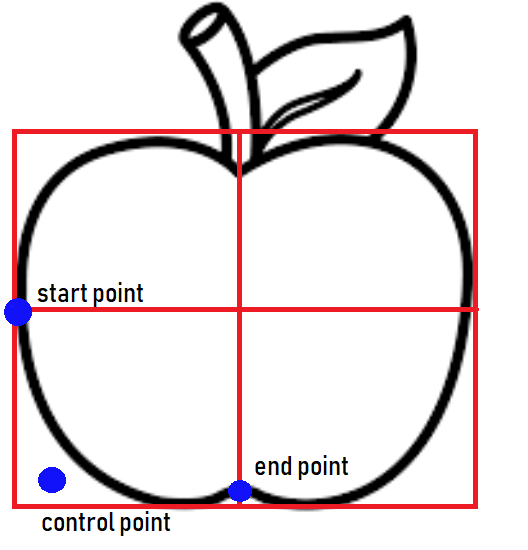
\includegraphics[scale=0.38]{apel4}
		\label{fig:apel4} 
	\end{minipage}
\end{figure}

\textbf{Pergerakan Ular}\\
Untuk membuat ular bergerak maju, dilakukan penambahan kepala dan pembuangan ekor secara bersamaan ketika ular sedang bergerak maju. Ilustrasinya dapat dilihat pada Gambar~\ref{fig:snakeMoveForward}. Untuk membuat ular bergerak dengan menggunakan cara pada Gambar~\ref{fig:snakeMoveForward}, algoritmanya adalah sebagai berikut : Pertama, semua elemen array akan dishift/digeser dan elemen pertama akan digantikan dengan koordinat yang baru. Setelah itu dilakukan pengecekan apakah panjang tubuh ular lebih besar dari jumlah elemen array tubuh ular. Jika benar, maka tidak dilakukan pembuangan elemen terakhir dan jika salah, maka tidak akan dilakukan apa-apa. 

\begin{figure}[H]
	\centering  
	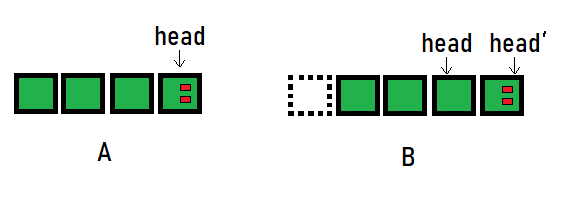
\includegraphics[scale=0.5]{snakeMoveForward}  
	\caption[Ilustrasi ular sebelum bergerak maju(A) dan setelah bergerak maju(B)]{Ilustrasi ular sebelum bergerak maju(A) dan setelah bergerak maju(B)}
	\label{fig:snakeMoveForward} 
\end{figure}

Kecepatan ular pada permainan ini adalah 1 sampai 5 \textit{pixel per frame}. Kecepatan maksimal ular tidak boleh melebihi lebar tubuh ular. Jika kecepatanya melebihi lebar ular, maka ketika terjadi tabrakan dengan tubuhnya sendiri, kepala ular tidak akan bertabrakan dengan tubuhnya. Kepala ular akan terlihat seolah-olah melompati tubuhnya sendiri. Dalam permainan ini, kecepatan ular adalah 2 \textit{pixel per frame}, karena dengan kecepatan 1 \textit{pixel per frame}, ular terlihat bergerak lebih lambat.\\

Ular dapat berbelok dengan menggunakan tombol pada \textit{keyboard}. Tombol ke kiri akan membuat ular bergerak melawan arah jarum jam dan tombol ke kanan akan membuat ular akan bergerak searah jarum jam. Pada permainan yang akan dibuat ini, digunakan sudut sebagai nilai untuk membuat ular dapat bergerak 360$^\circ$. Jika menekan tombol ke kiri maka sudut akan berkurang dan jika menekan tombol ke kanan maka sudut akan bertambah. Ketika menambahkan dan mengurangi sudut, perlu dilakukan pengecekan apabila nilai sudut valid atau tidak. Karena nilai sudut yang valid adalah antara nilai 0 sampai 360, maka apabila nilai sudut kurang dari 0, ubahlah sudut tersebut menjadi 360 dan apabila nilai sudut lebih besar dari 360, ubahlah nilai sudut tersebut menjadi 0. Dibutuhkan rumus trigonometri untuk menentukan posisi kepala ular. Untuk menghitung posisi koordinat x, digunakan \textit{sinus} sedangkan untuk menghitung posisi koordinat y menggunakan \textit{cosinus}. Lalu koordinat x dan y pada kepala ular akan ditambahkan dengan hasil perhitungan \textit{cosinus} dan \textit{sinus}.\\

\textbf{Labirin}\\
Dinding labirin akan dibuat dengan menggunakan garis. Cara pembuatanya sama dengan membuat tubuh ular yaitu dengan menggunakan titik-titik yang dihubungkan dengan garis yang pendek. Semua titik-titik tersebut akan disimpan pada sebuah array. Dinding labirin dapat juga dibuat dengan menggunakan kurva dikarenakan pergerakan ular yang sudah dapat bergerak 360$^\circ$. Level pada labirin dapat ditentukan berdasarkan kerumitan labirin. Labirin yang memiliki dinding yang banyak dan kompleks akan mendapatkan level yang lebih tinggi dibandingkan dengan labirin yang memiliki sedikit dinding dan lebih simpel. \\

\textbf{Pengecekan tabrakan(\textit{Collision Detection})}\\
Pada permainan ini terdapat pengecekan tabrakan yang dapat mengecek apakah ular sudah memakan makanan, ular menabrak tubuhnya sendiri, dan ular menabrak dinding labirin. Seluruh pengecekan ini akan dilakukan pada setiap \textit{frame}. Pada pengecekan tabrakan pada apel dan ular, hanya perlu mengecek tabrakan antara kepala ular dengan apel. Karena jalur yang dilalui oleh kepala ular, akan selalu dilalui oleh bagian tubuh ular. Dengan kata lain, bagian tubuh ular akan mengikuti ke mana kepala ular akan bergerak. Dengan ini, tidak perlu dilakukan \textit{collision detection} antara bagian tubuh ular dengan apel. Cukup hanya dengan mengecek tabrakan antara kepala ular dengan apel saja. Untuk mengetahui terjadinya tabrakan antara ular dengan apel, maka akan dibuat daerah tabrakan pada apel. Daerah tabrakan ini digunakan untuk mengecek apakah 2 benda saling bertabrakan satu sama lain. Daerah tabrakan pada apel ditandai dengan arsiran bewarna merah yang terdapat pada Gambar~\ref{fig:apelArsir}. Namun, untuk membuat daerah tabrakan ini cukup sulit ketika mengecek adanya tabrakan antara ular dengan apel terutama pada bagian lengkungan pada apel. Karena itu, daerah tabrakan pada apel dibuat dengan menggunakan bentuk persegi seperti pada Gambar~\ref{fig:apelArsirPersegi}. Jika posisi kepala ular berada di dalam daerah tabrakan apel, maka dipastikan bahwa ular tersebut sudah memakan apel. Algoritma untuk mengecek tabrakan adalah sebagai berikut : cek apakah koordinat x dari kepala ular lebih besar dari posisi sisi kiri daerah tabrakan dan lebih kecil dari posisi sisi kanan daerah tabrakan. Kemudian cek apakah koordinat y dari kepala ular lebih besar dari posisi sisi atas daerah tabrakan dan lebih kecil dari posisi sisi bawah daerah tabrakan. Jika posisi kepala ular berada memenuhi ketentuan tersebut, maka kepala ular berada di dalam daerah tabrakan apel.\\

\begin{figure}[H]
	\centering
	\begin{minipage}{.45\textwidth}
		\caption[Koordinat bagian tubuh ular pada \textit{array}]{Koordinat bagian tubuh ular pada \textit{array}}
		\centering
		\captionsetup{width=.3\textwidth}
		
\includegraphics[scale=0.38]{apelArsir}
		\label{fig:apelArsir} 
	\end{minipage}%
	\hfill
	\begin{minipage}{.45\textwidth}
		\caption[Tubuh ular setelah digambar menggunakan garis]{Tubuh ular setelah digambar menggunakan garis}
		\centering
		\captionsetup{width=.3\textwidth}
		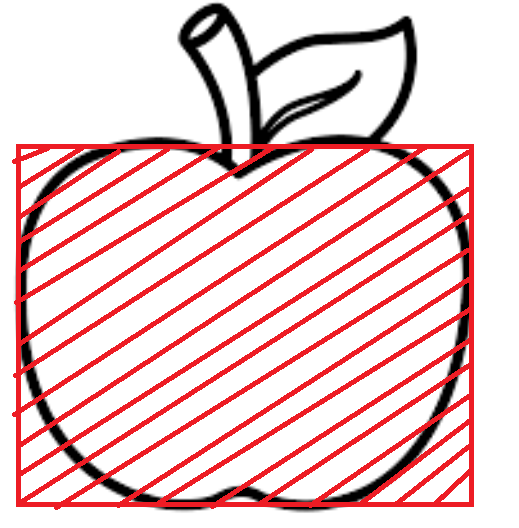
\includegraphics[scale=0.38]{apelArsirPersegi}
		\label{fig:apelArsirPersegi} 
	\end{minipage}
\end{figure}

Untuk mengecek tabrakan antara ular dengan tubuhnya sendiri adalah dengan mengecek tabrakan antara kepala ular dengan seluruh bagian tubuh ular. Algoritma pengecekanya adalah sebagai berikut : jika koordinat x kepala ular lebih kecil dari koordinat x bagian tubuh ular dikurangi panjang dari bagian tubuh ular dan lebih besar dari koordinat x bagian tubuh ular ditambah dengan panjang dari bagian tubuh ular. Kemudian dicek apabila koordinat y kepala ular lebih kecil dari koordinat y bagian tubuh ular dikurangi panjang dari bagian tubuh ular dan lebih besar dari koordinat y bagian tubuh ular ditambah dengan panjang dari bagian tubuh ular. Apabila posisi kepala ular memenuhi ketentuan tersebut, maka posisi kepala ular berada di dalam daerah tabrakan pada sebuah bagian tubuh ular. \\

Untuk mengecek tabrakan dengan labirin, algoritmanya sama dengan mengecek tabrakan antara ular dengan tubuh ular. Karena cara pembuatan labirin sama hampir sama dengan cara pembuatan tubuh ular, maka dilakukan pengecekan antara kepala ular dengan setiap dinding labirinya.

\end{itemize}

		\item \textbf{Merancang algoritma untuk menggambar tubuh ular, pergerakan ular dan membuat labirin.}\\
		{\bf Status :} Ada sejak rencana kerja skripsi.\\
		{\bf Hasil :} Sudah tercakup pada poin 2

		\item \textbf{Mengimplementasikan keseluruhan algoritma.}\\
		{\bf Status :} Ada sejak rencana kerja skripsi.\\
		{\bf Hasil :} Belum ada perkembangan.

		\item \textbf{Menambahkan labirin menggunakan \textit{pull request} pada \textit{Github}.}\\
		{\bf Status :} Ada sejak rencana kerja skripsi.\\
		{\bf Hasil :} Belum ada perkembangan.

		\item \textbf{Melakukan pengujian dan \textit{debugging}.}\\
		{\bf Status :} Ada sejak rencana kerja skripsi.\\
		{\bf Hasil :} Belum ada perkembangan.
		
		\item \textbf{Menulis dokumen skripsi} \\
		{\bf Status :} Ada sejak rencana kerja skripsi.\\
		{\bf Hasil :} Dokumen skripsi sudah ditulis sampai bab 3. Bab 1 berisikan latar belakang, rumusan masalah, tujuan, batasan masalah, metodologi, dan sistematika pembahasan dari penelitian yang dilakukan. Bab 2 berisikan dasar-dasar teori yang menunjang penelitian ini yaitu: pengertian \textit{Snake}, HTML5 Canvas, \textit{Javascript}, \textit{jQuery}, dan \textit{Git}. Bab 3 berisikan analisis sistem yang sudah ada, analisis sistem yang dibangun dan analisis berorientasi objek.

	\end{enumerate}

\section{Pencapaian Rencana Kerja}
Langkah-langkah kerja yang berhasil diselesaikan dalam Skripsi 1 ini adalah sebagai berikut:
\begin{enumerate}
\item Melakukan studi literatur tentang HTML5, \textit{JavaScript}, \textit{jQuery} dan \textit{Git}.
\item Melakukan analisis dan menentukan objek-objek pada \textit{Snake} 360.
\item Merancang algoritma untuk menggambar tubuh ular, pergerakan ular dan membuat labirin.
\item Menulis dokumen skripsi sampai bab 3.
\end{enumerate}



\section{Kendala yang Dihadapi}
%TULISKAN BAGIAN INI JIKA DOKUMEN ANDA TIPE A ATAU C
Kendala - kendala yang dihadapi selama mengerjakan skripsi :
\begin{itemize}
	\item Terlalu banyak tugas baik individu maupun kelompok dari mata kuliah lain sehingga pengerjaan skripsi menjadi terhambat.
	\item Terlalu banyak godaan berupa hiburan terutama game.
\end{itemize}

\vspace{1cm}
\centering Bandung, \tanggal\\
\vspace{2cm} \nama \\ 
\vspace{1cm}

Menyetujui, \\
\ifdefstring{\jumpemb}{2}{
\vspace{1.5cm}
\begin{centering} Menyetujui,\\ \end{centering} \vspace{0.75cm}
\begin{minipage}[b]{0.45\linewidth}
% \centering Bandung, \makebox[0.5cm]{\hrulefill}/\makebox[0.5cm]{\hrulefill}/2013 \\
\vspace{2cm} Nama: \pembA \\ Pembimbing Utama
\end{minipage} \hspace{0.5cm}
\begin{minipage}[b]{0.45\linewidth}
% \centering Bandung, \makebox[0.5cm]{\hrulefill}/\makebox[0.5cm]{\hrulefill}/2013\\
\vspace{2cm} Nama: \pemB \\ Pembimbing Pendamping
\end{minipage}
\vspace{0.5cm}
}{
% \centering Bandung, \makebox[0.5cm]{\hrulefill}/\makebox[0.5cm]{\hrulefill}/2013\\
\vspace{2cm} Nama: \pembA \\ Pembimbing Tunggal
}
\end{document}

